%%
%% Expert Systems with Applications — Elsevier Submission
%% elsarticle template with numerical citations
%%
\documentclass[12pt,number]{elsarticle}

%% Packages
%\usepackage{lineno} % Disabled for final submission
\usepackage{setspace} % Added for spacing control
\usepackage{times} % Professional font
\usepackage[utf8]{inputenc}
\usepackage[T1]{fontenc}
\usepackage{lscape} % Landscape pages
\usepackage{amsmath,amssymb,amsfonts}
\usepackage{amsthm}
\usepackage{graphicx}
\usepackage{booktabs}
\usepackage{multirow}
\usepackage{xcolor}
\usepackage{array}
\usepackage{hyperref}
\usepackage{algorithm}
\usepackage{algpseudocode}
\usepackage{subcaption}
\usepackage{float}
\usepackage{placeins}

%% Page geometry for compact format
\usepackage{geometry}
\geometry{margin=1in,top=0.9in,bottom=0.9in}

%% Compact spacing
\setlength{\parskip}{0pt}
\setlength{\parindent}{0.15in}
\linespread{0.96}

%% Analytical Statement environments
\newtheorem{empiricalproperty}{Empirical Property}
\newtheorem{corollary}{Corollary}
\newtheorem{definition}{Definition}
\newtheorem{observation}{Observation}
\renewcommand{\proofname}{Analytical Explanation}

%% Journal metadata
\journal{Expert Systems with Applications}

\begin{document}

\begin{frontmatter}

\title{Hybrid CP-SAT and Quantum-Inspired Optimization for Airline Disruption Recovery with Explainable Decision Support}

\author[cska]{K\"ur\c{s}at Kahya\corref{cor1}}
\ead{kahyakursat1@gmail.com}
\cortext[cor1]{Corresponding author.}
\address[cska]{Department of Aviation and Space Sciences, \c{C}ukurova Science and Art Center, Adana, T\"urkiye}

\begin{abstract}
Airline disruption recovery operates under uncertainty: crew locations are imprecise, weather forecasts erroneous, and passenger connections cascade-fragile. Classical exact solvers (CP-SAT) guarantee nominal optimality but time out under uncertainty; metaheuristics run fast but risk regulatory violations. This paper maps the problem into four regimes governed by CP-SAT's residual optimality gap and the level of uncertainty: (i)~\emph{deterministic, CP-SAT converged} (RealCal-300, gap $=0$): CP-SAT closes the problem in $\sim$10\,ms and warm-started QIGA introduces a bounded $-0.7\%$ regression; (i')~\emph{deterministic, CP-SAT gap-bounded} (Baseline-150, residual gap $\approx 2\%$): warm-started QIGA exploits the gap and improves the objective by $\sim 5\%$; (ii)~\emph{stochastic uncertain} (50--100 flights with crew/weather/connection uncertainty): CP-SAT exhausts its budget without returning a feasible solution, while QIGA delivers solutions feasible across 90--92\% of adverse scenarios in $<$5\,s; (iii)~\emph{multi-day large-scale} (up to 1{,}617 flights over 12 days): monolithic CP-SAT runs out of memory and rolling-horizon decomposition becomes the only practical path. The methodological contribution is a warm-start mechanism that initialises a quantum-inspired genetic algorithm from CP-SAT's feasible solution and uses generational elitist selection---a safety pattern that \emph{preserves feasibility unconditionally} and \emph{bounds worst-case objective regression} ($-0.7\%$ in our experiments) rather than guaranteeing strict monotonic improvement. A bidirectional explainability layer couples SHAP feature importance from an XGBoost pre-diagnostic model to the constraints those features modulate, exposing a single causal chain (feature $\rightarrow$ constraint $\rightarrow$ decision) that targets the traceability requirement of EASA AMC 20-42.
\end{abstract}

\begin{keyword}
Airline Disruption Management \sep Constraint Programming \sep CP-SAT \sep Quantum-Inspired Genetic Algorithm \sep Explainable AI \sep SHAP \sep EASA Flight Time Limitations \sep Irregular Operations
\end{keyword}

\end{frontmatter}

%% Final submission format (no double spacing, no line numbers)

%% ============================================================
%%  1. INTRODUCTION
%% ============================================================
\section{Introduction}
\label{sec:introduction}

Global aviation carried 4.5 billion passengers in 2023, executing 8.8 million flights \cite{iata2024}. This massive operational scale masks a persistent vulnerability: when something goes wrong---a mechanical failure, weather delay, or crew absence---the recovery problem becomes urgent and severely constrained \cite{hu2024}. Decisions must be made in minutes, not hours. The U.S. alone incurs roughly \$33 billion annually in delay costs \cite{ball2010}, much of it driven by suboptimal real-time crew and aircraft assignments rather than external factors \cite{barnhart2004}. One crew member's delayed arrival cascades through a dozen downstream flights; one aircraft swap can enable or block dozens of connections. The challenge is fundamentally combinatorial: thousands of possible reassignments, hundreds of hard constraints (crew duty hours, aircraft maintenance, gate conflicts), and a ticking clock.

A critical but understudied challenge is \textbf{uncertainty}: recovery decisions are made with incomplete information. Crew locations during disruption are imprecise, weather forecasts are uncertain, and downstream passenger connections may fail in unforeseen ways. A nominally optimal recovery schedule may be infeasible under real-world uncertainty. Robust optimization addresses this: find solutions that are feasible and near-optimal across a range of adverse scenarios, not just the nominal case.

Two classes of algorithms address optimization under time pressure and uncertainty: exact methods (MILP, constraint programming, robust optimization) and metaheuristics (genetic algorithms, evolutionary search). Exact methods guarantee feasibility under nominal conditions but often timeout on large instances---a 500-flight recovery problem can exceed 60 seconds on standard hardware, especially with uncertainty quantification. Metaheuristics find good solutions quickly and can explore robust alternatives under uncertainty, but risk producing schedules that violate crew duty regulations or crew continuity constraints, rendering them operationally inadmissible in a regulated industry. Neither approach alone is sufficient for robust disruption recovery.

Recent constraint programming solvers like Google OR-Tools CP-SAT (Constraint Programming - Satisfiability) achieve impressive performance on scheduling benchmarks \cite{perron2023,laborie2018}, and quantum-inspired evolutionary algorithms (QIGA) have shown promise in other domains \cite{zhang2011}. But combining them productively is non-trivial. Simply running a genetic algorithm after a timeout is reckless: it can easily violate the constraints the exact solver worked hard to satisfy. We address this fundamental challenge by demonstrating that seeding QIGA from a CP-SAT solution preserves feasibility by construction (the population is initialised inside the feasible region and generational elitism keeps it there) and bounds the worst-case objective regression to a small margin, while exploring for improvement when CP-SAT has left a residual optimality gap. This warm-start mechanism is empirically validated across all five instance families defined in Table~\ref{tab:instances}. This is the paper's core methodological contribution---a practically-grounded approach with immediate implications for deploying evolutionary algorithms in regulated domains (aviation, power grids, telecommunications).

A second challenge is explainability. Regulators increasingly demand transparency. The European Union Aviation Safety Agency (EASA) AMC 20-42 guidance (Acceptable Means of Compliance 20-42) on AI in aviation requires that decisions be traceable and explainable \cite{easa2023}. A pure black-box genetic algorithm fails this requirement; so does a constraint program that produces only a schedule with no rationale. We address this by creating an explicit bidirectional mapping between optimization constraints and SHAP feature importance, allowing us to explain both \emph{which features mattered} and \emph{which constraints they triggered}.

Our main contributions are:

(1)~\textbf{Operational regime delineation tied to CP-SAT's optimality gap:} We identify and empirically map four regimes in airline disruption recovery, controlled by whether CP-SAT converges within the time budget and how much uncertainty is present: (i)~\emph{deterministic, CP-SAT converged} (RealCal-300, residual gap $=0$): CP-SAT closes the problem in $\sim$10\,ms and warm-started QIGA introduces a bounded objective regression of $-0.7\%$; (i')~\emph{deterministic, CP-SAT gap-bounded} (Baseline-150, 60\,s budget, residual gap $\approx$2\%): warm-started QIGA exploits the residual gap and improves the objective by $\sim$5\% over CP-SAT alone; (ii)~\emph{stochastic uncertain} (Stochastic-50/100 with crew/weather/connection uncertainty): CP-SAT exhausts its budget without returning a feasible solution, while QIGA delivers feasible solutions across 90--92\% of adverse scenarios in $<$5\,s; (iii)~\emph{multi-day large-scale} (Scale-8d/12d, $\geq$1{,}100 flights): monolithic CP-SAT runs out of memory in conflict-clause learning and rolling-horizon decomposition is required. The key empirical observation is that hybrid value tracks CP-SAT's residual optimality gap: when the gap is zero, refinement only risks bounded regression; when the gap is non-trivial, refinement closes it. This regime map replaces vague hybrid-vs-exact claims with quantified boundaries and is the most actionable methodological contribution of the paper.

(2)~\textbf{Warm-start safety pattern for regulated metaheuristic search:} We adapt the quantum-inspired evolutionary algorithm of Han \& Kim~\cite{han2002} as a refinement layer and show that seeding its initial population with a CP-SAT feasible solution, combined with elitist selection, \emph{preserves feasibility unconditionally} (the CP-SAT solution is retained in every generation) while \emph{bounding the worst-case objective regression} to a small margin (observed worst case: $-0.7\%$ on instances where CP-SAT already converges). This bounded-regression property---not strict monotonic improvement, which the data does not support on already-converged instances---is what makes the refinement step safe enough to deploy in regulated settings, where infeasible schedules are operationally unusable.

(3)~\textbf{EASA-compliant optimization model} enforcing crew duty regulations (CAT.OP.MPA.210) via a conservative 600-minute proxy, validated through a sensitivity analysis (Table~\ref{tab:ftl_sensitivity}) and a systematic stress evaluation on a real Turkish Airlines route network (SysVal-140, five disruption types).

(4)~\textbf{Bidirectional explainability layer} that couples SHAP feature importance from an XGBoost \emph{pre-diagnostic} model to the CP-SAT constraints those features modulate, producing a single causal chain (feature $\rightarrow$ constraint $\rightarrow$ decision reason) intended to address the traceability requirements of EASA AMC 20-42.

(5)~\textbf{End-to-end validation across five instance families} (Table~\ref{tab:instances}): Baseline-150 (synthetic deterministic, 1 day), RealCal-300 (IATA-calibrated deterministic, 1 day), Stochastic-50/100 (explicit crew/weather/connection uncertainty), SysVal-140 (real Turkish Airlines route network, five operational disruption types), and Scale-1/4/8/12d (multi-day scalability up to 1{,}617 flights). Worst-case stress conditions are applied as an overlay scenario on the Baseline-150 family (Table~\ref{tab:worstcase}), not as a separate instance family.

The rest of the paper is organized as: Related Work (Section~\ref{sec:related}), Problem Formulation (Section~\ref{sec:formulation}), Hybrid Framework (Section~\ref{sec:framework}), Explainability Layer (Section~\ref{sec:xai}), Experimental Results (Section~\ref{sec:experiments}), Discussion (Section~\ref{sec:discussion}), and Conclusion (Section~\ref{sec:conclusion}).


%% ============================================================
%%  2. RELATED WORK
%% ============================================================
\section{Related Work}
\label{sec:related}

The airline disruption-recovery literature can be organised along three axes that are directly relevant to our framework: (i)~exact optimisation methods that guarantee feasibility but scale poorly, (ii)~metaheuristic and learning-based methods that scale well but cannot guarantee regulatory compliance, and (iii)~explainability techniques that historically target machine-learning models rather than discrete optimisation outputs. We review each in turn and then position our contribution.

\subsection{Exact Methods for Airline Recovery}

Airline planning has long been dominated by mathematical-programming approaches. Column generation for crew pairing~\cite{barnhart1998,desrosiers2005} and integer programming for fleet assignment~\cite{abara1989,hane1995,rexing2000,sherali2006} guarantee global optimality and remain the reference techniques for tactical planning. For \emph{recovery} (as opposed to planning), aircraft rerouting integer programs~\cite{rosenberger2003}, real-time crew rescheduling~\cite{stojkovic2002}, and stochastic crew programming~\cite{yen2006} extend the planning toolkit to disruption scenarios. The trade-off is well documented: a 500-flight recovery problem solved with modern MILP solvers typically consumes tens of minutes, which is incompatible with operational time pressure~\cite{ball2007,hu2024}.

For broader background on operations research in commercial aviation, see Barnhart et al.'s survey~\cite{barnhart2003}. Constraint programming (CP) provides better modelling expressiveness and tighter pruning than MILP on scheduling problems~\cite{rossi2006,laborie2018}. Recent CP-SAT solvers~\cite{perron2023} combine SAT-style conflict learning with LP relaxations and have closed previously open scheduling benchmarks, but exponential worst-case complexity remains and conflict-clause memory becomes a binding constraint above roughly $10^3$ flights, as we confirm empirically in Section~\ref{sec:scalability}.

\subsection{Metaheuristic and Learning-based Methods}

Genetic algorithms have been applied to crew scheduling for decades~\cite{levine1996,ozdemir2001} and to airline disruption recovery in more recent hybrid multi-objective form~\cite{liu2010}. Quantum-inspired evolutionary algorithms (QIEA) originate with Han \& Kim~\cite{han2002} and were surveyed by Zhang~\cite{zhang2011}; we are not aware of a published application of QIEA specifically to airline schedule recovery prior to this work, so the present paper also serves as the first such transfer. The common limitation of all these methods, with or without quantum-inspired encoding, is the same: without an exact-solver back-stop they cannot guarantee that the returned schedule satisfies hard regulatory constraints such as EASA CAT.OP.MPA.210. In a regulated industry, an infeasible solution is operationally unusable regardless of its objective value.

Parallel to the optimisation literature, machine learning has been used to \emph{predict} delays and disruption propagation rather than to compute recoveries~\cite{ahmadbeygi2008,gui2020,jacquillat2015}. Predictive models offer fast inference but no feasibility guarantees, so they are typically used as inputs to a downstream optimiser rather than as a replacement for it. Our framework follows this pattern: the XGBoost~\cite{chen2016} pre-diagnostic provides risk signals that feed Table~\ref{tab:xai_coupling}, while CP-SAT remains responsible for the feasibility-bearing decisions.

\subsection{Explainability for Optimisation Decisions}

Explainability methods such as LIME~\cite{ribeiro2016}, SHAP~\cite{lundberg2017}, TreeSHAP~\cite{lundberg2020}, and counterfactual explanations~\cite{wachter2018} were developed for learned models; their assumptions (gradients, feature additivity, sampling-based perturbation) do not transfer cleanly to discrete optimisation outputs. The broader XAI taxonomy~\cite{arrieta2020} treats interpretation of constraint-programming decisions as a largely open problem, and recent benchmarking work has shown that anecdotal explanations of black-box models do not generalise across tasks~\cite{nauta2023}. As a result, very few airline-optimisation papers report any explanation alongside their schedules; when they do, it is typically a textual rationale generated after the fact rather than a traceable mapping from input features to binding constraints.

\subsection{The Gap and How This Paper Addresses It}

Prior work falls into two camps---exact solvers that guarantee feasibility but timeout, and fast heuristics that find good solutions but risk infeasibility---and treats explainability as an afterthought, if at all. Three concrete gaps remain: (G1)~no published study delineates \emph{when} a hybrid exact/metaheuristic approach actually outperforms the exact solver alone for airline recovery, (G2)~the safety properties of warm-starting a metaheuristic from an exact-solver solution have not been empirically characterised in a regulated setting, and (G3)~SHAP-style feature attribution has not been wired to the constraints it modulates, so feature importance and decision causes are reported as two parallel justifications instead of a single causal chain. The remainder of the paper targets these three gaps in order.

Table~\ref{tab:lit} provides a comparative positioning of the proposed approach.

\begin{table}[H]
\centering
\caption{Comparative positioning of the proposed approach in the literature. \emph{Abbreviations:} CBLS = Constraint-Based Local Search; IROPS = Irregular Operations (disruption recovery); QIGA = Quantum-Inspired Genetic Algorithm.}
\label{tab:lit}
\small
\begin{tabular}{@{}llllllc@{}}
\toprule
\textbf{Approach} & \textbf{Source} & \textbf{Problem} & \textbf{Scale} & \textbf{Time} & \textbf{Optimality} & \textbf{XAI} \\
\midrule
Column Generation & \cite{barnhart1998} & Crew pairing & $\leq$5000 & Hours & Global & --- \\
MILP (Gurobi) & \cite{rexing2000} & Fleet assign. & $\leq$2000 & Minutes & Global & --- \\
CP + CBLS & \cite{laborie2018} & Scheduling & Medium & Minutes & Near-opt. & --- \\
GA (multi-obj.) & \cite{levine1996,liu2010} & Recovery / crew & Medium & Seconds & Heuristic & --- \\
QIEA & \cite{han2002,zhang2011} & Combinatorial & Variable & Seconds & Heuristic & --- \\
ML prediction & \cite{gui2020} & Delay prop. & Network & Offline & Predictive & --- \\
Rerouting IP & \cite{rosenberger2003} & Recovery & Medium & Minutes & Near-opt. & --- \\
\textbf{This paper} & --- & \textbf{IROPS} & $\leq$\textbf{500} (1\,d) / \textbf{1{,}617} (RH, 12\,d) & $\leq$\textbf{60\,s} & \textbf{CP+QIGA} & \checkmark \\
\bottomrule
\end{tabular}
\end{table}


%% ============================================================
%%  3. PROBLEM FORMULATION
%% ============================================================
\section{Problem Formulation}
\label{sec:formulation}

\subsection{Problem Description}

Disruption recovery operates under uncertainty: when a disruption occurs (e.g., weather, mechanical failure, crew illness), recovery decisions must be made with incomplete information. Uncertainty arises from:

\begin{itemize}
    \item \textbf{Crew location uncertainty:} Crew positions during disruption are imprecise (cell phone data, last known location, potential multi-leg disruption).
    \item \textbf{Weather forecast error:} Future weather is uncertain; recovery must account for possible worsening or improvement.
    \item \textbf{Passenger connection viability:} Downstream flight connections may be disrupted; recovery must be robust to cascading failures.
    \item \textbf{Aircraft availability:} Mechanical status, maintenance, and potential secondary faults are uncertain.
\end{itemize}

Recovery decisions must therefore balance two competing objectives: (1)~maximize robustness to uncertainty (avoid solutions that fail under adverse scenarios), and (2)~optimize profit under nominal conditions. The problem couples three subproblems under uncertainty: (1)~which aircraft operates each flight, (2)~which crew is assigned, (3)~how much delay is absorbed. All assignments must respect hard constraints: an aircraft can't be in two places, a crew member can't exceed their duty limit, passenger connections require minimum ground time. We model this as a robust constraint satisfaction problem with a stochastic optimization objective: maximize expected profit while maintaining feasibility across uncertain disruption outcomes.

\subsection{Sets and Decision Variables}

Let $F$, $K$, and $C$ denote the sets of flights, aircraft, and crew, respectively, with $A$ denoting the set of airports and $T$ the set of time slots (15-minute intervals).

\begin{table}[H]
\centering
\small
\caption{Decision variables of the CP-SAT model.}
\label{tab:vars}
\begin{tabular}{@{}clll@{}}
\toprule
\textbf{Symbol} & \textbf{Type} & \textbf{Description} & \textbf{Domain} \\
\midrule
$x_{f,k}$ & Binary & Flight $f$ assigned to aircraft $k$ & $f \in F, k \in K$ \\
$y_{f,c}$ & Binary & Flight $f$ assigned to crew $c$ & $f \in F, c \in C$ \\
$z_f$ & Binary & Flight $f$ is cancelled & $f \in F$ \\
$d_f$ & Integer & Delay assigned to flight $f$ (min) & $0 \leq d_f \leq D_{\max}$ \\
$\delta_f$ & Integer & Actual departure time of $f$ & --- \\
$g_{f,a,t}$ & Binary & $f$ uses a gate at airport $a$, time $t$ & $f \in F,\ a \in A,\ t \in T$ \\
\bottomrule
\end{tabular}
\end{table}

\subsection{Constraints}

The model enforces ten constraint families ensuring operational feasibility and regulatory compliance (Table~\ref{tab:constraints}).

\begin{table}[H]
\centering
\caption{Constraint families.}
\label{tab:constraints}
\small
\begin{tabular}{@{}llll@{}}
\toprule
\textbf{Constraint} & \textbf{ID} & \textbf{Description} & \textbf{Type} \\
\midrule
Assignment uniqueness & C$_1$ & Each flight $\to$ at most one aircraft & Hard \\
Crew uniqueness & C$_2$ & Each flight $\to$ at most one crew & Hard \\
Aircraft capacity & C$_3$ & Capacity $\geq$ passenger count & Hard \\
Aircraft continuity & C$_4$ & Same aircraft connects at same airport & Hard \\
Crew continuity & C$_5$ & Same crew connects at same airport & Hard \\
EASA FTL & C$_6$ & Crew cumulative block time $\leq 600$ min & Hard \\
Gate capacity & C$_7$ & Max $G_a$ aircraft/airport/time slot & Hard \\
Slot capacity & C$_8$ & Hourly movements $\leq$ airport capacity & Hard \\
Min.\ Connection Time & C$_9$ & Passenger connection $\geq$ MCT & Hard \\
Cancel consistency & C$_{10}$ & Cancelled $\Rightarrow$ no assignments & Hard \\
\bottomrule
\end{tabular}
\end{table}

\textbf{(C$_1$) Assignment uniqueness:}
\begin{equation}
\sum_{k \in K} x_{f,k} + z_f = 1, \quad \forall f \in F
\label{eq:c1}
\end{equation}

\textbf{(C$_2$) Crew uniqueness:}
\begin{equation}
\sum_{c \in C} y_{f,c} \leq 1 - z_f, \quad \forall f \in F
\label{eq:c2}
\end{equation}

\textbf{(C$_3$) Aircraft capacity:}
\begin{equation}
\sum_{k \in K} \mathrm{cap}_k \cdot x_{f,k} \geq \mathrm{pax}_f \cdot (1 - z_f), \quad \forall f \in F
\label{eq:c3}
\end{equation}

\textbf{(C$_4$) Aircraft continuity:} For consecutive flights $f_1, f_2$ on the same aircraft $k$:
\begin{equation}
x_{f_1,k} + x_{f_2,k} \leq 1 \quad \text{if } \mathrm{dest}_{f_1} \neq \mathrm{orig}_{f_2}
\label{eq:c4}
\end{equation}

\textbf{(C$_5$) Crew continuity:} For consecutive flights $f_1, f_2$ on the same crew $c$:
\begin{equation}
y_{f_1,c} + y_{f_2,c} \leq 1 \quad \text{if } \mathrm{dest}_{f_1} \neq \mathrm{orig}_{f_2}
\label{eq:c5}
\end{equation}

\textbf{(C$_6$) EASA FTL (conservative proxy):}
\begin{equation}
\sum_{f \in F} y_{f,c} \cdot \mathrm{block}_f \leq \bar{B}, \quad \forall c \in C,
\label{eq:c6}
\end{equation}
\noindent where $\bar{B} = 600$ min is used as a \emph{conservative uniform ceiling} derived from the tightest single-crew-type entry of EASA CAT.OP.MPA.210~\cite{easa2022} under a one-sector, non-WOCL scenario. This proxy is deliberately restrictive: any schedule satisfying~\eqref{eq:c6} is also feasible under the full FDP$\times$sector$\times$WOCL matrix, so the model cannot produce FTL violations when the complete table is substituted. We retain~\eqref{eq:c6} in the main experiments because it preserves the combinatorial structure exercised by CP-SAT while yielding a regulator-safe over-approximation; a richer table-driven formulation is a drop-in replacement that we discuss in Section~\ref{sec:discussion}.

\textbf{(C$_7$) Gate capacity:} For each airport $a$ and time slot $t$, the number of flights occupying gates at $(a,t)$ cannot exceed the available gate count $G_a$:
\begin{equation}
\sum_{f \in F} g_{f,a,t} \leq G_a, \quad \forall a \in A,\ \forall t \in T
\label{eq:c7}
\end{equation}
where $g_{f,a,t} = 1$ if flight $f$ occupies a gate at airport $a$ during time slot $t$, linked to the assignment variables by $g_{f,a,t} \leq \sum_{k \in K} x_{f,k}$ for all $f \in F$, $a \in A$, $t \in T$, and forced to zero whenever $a$ is neither the origin nor the destination of $f$.

\textbf{(C$_8$) Airport slot capacity:} For each airport $a$ and hour $h$:
\begin{equation}
\sum_{f: \mathrm{dep}(f) \in h, \mathrm{orig}(f)=a} (1 - z_f) \leq \mathrm{Cap}_a(h)
\label{eq:c8}
\end{equation}

\textbf{(C$_9$) Minimum Connection Time:} For passenger connection $(f_{\mathrm{in}}, f_{\mathrm{out}})$:
\begin{equation}
\delta_{f_{\mathrm{out}}} - \bigl(\delta_{f_{\mathrm{in}}} + \mathrm{block}_{f_{\mathrm{in}}}\bigr) \geq \mathrm{MCT}_a \cdot (1 - z_{f_{\mathrm{in}}} - z_{f_{\mathrm{out}}})
\label{eq:c9}
\end{equation}

\textbf{(C$_{10}$) Cancel consistency:} If a flight is cancelled, it has no resource assignments:
\begin{equation}
\sum_{k \in K} x_{f,k} + \sum_{c \in C} y_{f,c} \leq (1 - z_f) \cdot (|K| + |C|)
\label{eq:c10}
\end{equation}

\subsection{Objective Function}

The objective minimizes total operational cost:
\begin{equation}
\min \sum_{f \in F} \Bigl[ \alpha \cdot z_f \cdot R_f + \beta \cdot d_f \cdot w_f + \gamma \sum_{k \in K} x_{f,k} \cdot \mathrm{fuel}_{f,k} + \mu \cdot z_f \cdot \mathrm{slotPen}_f \Bigr]
\label{eq:obj}
\end{equation}
where $R_f$ is the revenue loss from cancellation, $w_f$ is the delay cost per minute (weighted by passenger volume and connection criticality), $\mathrm{fuel}_{f,k}$ is the fuel cost, and $\alpha, \beta, \gamma, \mu$ are strategy-dependent weights (Table~\ref{tab:weights}).

\begin{table}[H]
\centering
\small
\caption{Strategy weight configurations.}
\label{tab:weights}
\begin{tabular}{@{}lcccc@{}}
\toprule
\textbf{Strategy} & $\alpha$ (cancel) & $\beta$ (delay) & $\gamma$ (fuel) & $\mu$ (slot) \\
\midrule
PROFIT & 1.0 & 1.0 & 0.3 & 0.5 \\
ECO & 0.8 & 1.2 & 1.5 & 0.4 \\
RESILIENCE & 1.5 & 0.8 & 0.4 & 1.0 \\
\bottomrule
\end{tabular}
\end{table}

\subsection{Complexity Analysis}

The model has $O(|F| \cdot (|K| + |C|))$ variables and $O(|F|^2)$ constraints. For the baseline experimental instance ($|F|=150$, $|K|=20$, $|C|=40$): ${\sim}9{,}000$ variables and ${\sim}22{,}500$ constraints. QIGA complexity: $O(G_{\max} \cdot N \cdot |F|)$. We use two QIGA budgets in the experiments: \emph{full-budget} ($N=50$, $G_{\max}=200$) for the main comparisons and ablation, and \emph{tactical-budget} ($N=20$, $G_{\max}=8$) for the stochastic instances where sub-second turnaround is required. Both configurations are reported per table.


%% ============================================================
%%  4. HYBRID OPTIMIZATION FRAMEWORK
%% ============================================================
\section{Hybrid Optimization Framework}
\label{sec:framework}

\subsection{Overview}

Our hybrid approach combines the strengths of two different algorithm families. First, we use an exact constraint solver (CP-SAT) to find a solution that definitely satisfies all regulatory constraints---it might not be globally optimal under tight time budgets, but it is feasible. Then, we use an evolutionary algorithm (QIGA) to explore nearby solutions and improve profit while staying within the feasible region established by the first stage. This two-stage approach addresses the core trade-off: exact solvers guarantee feasibility but may timeout on large instances, while evolutionary algorithms are fast but can violate constraints. By running them in sequence, initialized carefully, we obtain the safety of an exact solver and the timeout robustness of a metaheuristic.

\begin{figure}[!ht]
\centering
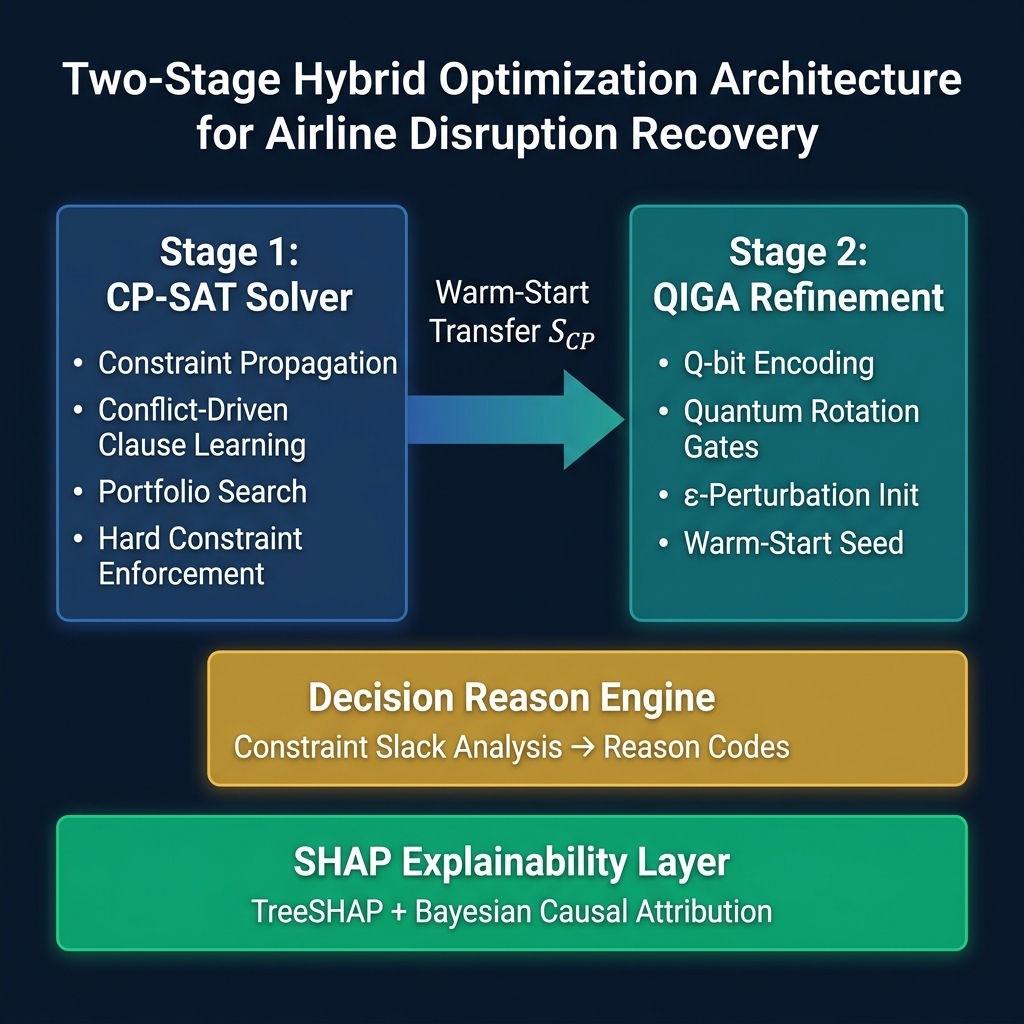
\includegraphics[width=\textwidth]{figures/fig1_hybrid_architecture.png}
\caption{Two-stage hybrid optimization architecture. The CP-SAT solver generates a feasible solution enforcing all hard constraints; QIGA refines it via quantum-rotation-gate-driven population evolution initialised with the CP-SAT solution. The same pipeline is exercised differently per regime (Table~\ref{tab:method_selection}): on instances where CP-SAT converges (gap $=0$) the refinement stage runs but produces at most a bounded objective regression; on instances with a residual CP-SAT gap, QIGA closes that gap; on instances where CP-SAT times out, QIGA runs from the best partial CP-SAT assignment available.}
\label{fig:architecture}
\end{figure}

\begin{algorithm}[!ht]
\caption{Hybrid CP-SAT + QIGA Framework}
\label{alg:hybrid}
\begin{algorithmic}[1]
\Require Flight schedule $\mathcal{F}$, aircraft set $\mathcal{A}$, crew set $\mathcal{K}$, constraints $\mathcal{C}$, time budget $T_{\max}=60\text{ s}$
\Ensure Feasible solution $S_{\mathrm{M}}$ with crew assignments, flight cancellations, and delay recommendations

\State{\textbf{Stage 1: Exact Feasibility via CP-SAT}}
\State{$S_{\mathrm{CP}} \gets \textsc{CP-SAT-Solve}(\mathcal{F}, \mathcal{A}, \mathcal{K}, \mathcal{C}, T_{\max})$}
\If{$S_{\mathrm{CP}}$ is feasible}
  \State{Initialize: $\text{best} \gets S_{\mathrm{CP}}$}
\Else
  \State{Log infeasibility; $\text{best} \gets \text{greedy heuristic}$}
\EndIf

\State{\textbf{Stage 2: Refinement via Warm-Started QIGA}}
\State{Initialize QIGA population: $\text{Pop}_0[0] \gets S_{\mathrm{CP}}$}
\State{Generate $N-1$ neighbors via $\epsilon$-perturbation: $\text{Pop}_0[1..N-1] \gets \text{Perturb}(S_{\mathrm{CP}}, \epsilon)$}
\State{Initialize Q-bits encoding $S_{\mathrm{CP}}$: $(\alpha, \beta) \gets (0.95, 0.31)$ \Comment{High $\alpha^2$ on bits matching $S_{\mathrm{CP}}$; biased decoding}}

\For{$g = 1$ to $G_{\max}$ (generations)}
  \For{each individual $\xi$ in $\text{Pop}_g$}
    \State{Evaluate: $\text{Fitness}[\xi] \gets \text{Profit}(\xi) - \lambda \cdot \text{Violations}(\xi)$}
    \State{Update Q-bits via rotation gate (Eq.~\ref{eq:rotation})}
  \EndFor
  \State{Select elite individual: $\text{best} \gets \operatorname{argmax}_{\xi \in \text{Pop}_g} \text{Fitness}[\xi]$}
  \State{Preserve $\text{best}$ in $\text{Pop}_{g+1}$ (elitist selection)}
\EndFor

\State{\Return $S_{\mathrm{M}} \gets \text{best}$ \Comment{Feasibility preserved unconditionally; objective bounded by Empirical Property~\ref{prop:warm}}}
\end{algorithmic}
\end{algorithm}

\subsection{Stage 1: CP-SAT Feasible Solution Generation}

The first stage uses Google OR-Tools CP-SAT, a modern constraint solver that combines integer programming relaxations with Boolean satisfiability techniques \cite{perron2023}. We allocate a 60-second time budget. Within this window, CP-SAT hunts for the best feasible assignment it can find, guaranteeing that all hard constraints (crew duty hours, aircraft continuity, passenger connections) are satisfied. When the timeout arrives, we take the best solution found so far, call it $S_{\mathrm{CP}}$, and pass it to Stage 2.

\subsection{Stage 2: Quantum-Inspired Genetic Algorithm (QIGA)}

Stage 2 runs the quantum-inspired evolutionary algorithm originally proposed by Han \& Kim~\cite{han2002} and surveyed by Zhang~\cite{zhang2011}. We make no claim of a new metaheuristic here; the contribution is in how QIGA is initialized and constrained, not in the rotation-gate update itself. The algorithm encodes each position with two amplitudes $(\alpha, \beta)$ rather than a single binary digit, which empirically slows the loss of population diversity relative to a classical binary GA (Section~\ref{sec:ablation_conv}).

Population evolution is driven by quantum rotation gates applied to the Q-bit representation:
\begin{equation}
\begin{pmatrix} \alpha'_i \\ \beta'_i \end{pmatrix} = \begin{pmatrix} \cos\Delta\theta & -\sin\Delta\theta \\ \sin\Delta\theta & \cos\Delta\theta \end{pmatrix} \begin{pmatrix} \alpha_i \\ \beta_i \end{pmatrix}
\label{eq:rotation}
\end{equation}
where $\Delta\theta$ is adaptively determined based on fitness differences, enabling exploration while concentrating search near high-quality regions.

For each flight, the algorithm can decide: keep the original assignment, add a delay, cancel, or swap aircraft. The population of $N = 50$ individuals evolves for $G_{\max} = 200$ generations under the default budget; a tactical short-budget configuration ($N = 20$, $G_{\max} = 8$) is also evaluated for sub-second refinement scenarios. Fitness is defined as:
\begin{equation}
\mathcal{F}(\xi) = \mathrm{Profit}(\xi) - \lambda \cdot \mathrm{Hard\text{-}Constraint\,Violations}(\xi)
\label{eq:fitness}
\end{equation}

A high $\lambda$ (penalty for violations) aims to keep solutions feasible during evolution. The adaptive rotation angle adjustments push the population toward high-fitness regions while maintaining diversity \cite{han2002}.

\subsection{Warm-Start: The Critical Link}

The key insight is how we initialise QIGA. Rather than starting with random solutions, we place $S_{\mathrm{CP}}$ as the first individual in the population and generate the remaining $N-1$ individuals as $\epsilon$-perturbations of $S_{\mathrm{CP}}$ (for the default budget, $N-1 = 49$; for the tactical budget, $N-1 = 19$). This seeding creates three structural conditions: (i)~the population is initialised inside the feasible region, (ii)~the evolutionary search never has to explore far from the CP-SAT solution, and (iii)~each generation's elite is retained (generational elitism) and the high-penalty fitness function ($\lambda \to \infty$ on hard-constraint violations) ranks every feasible chromosome strictly above every infeasible one, so the elite is always feasible and feasibility is preserved by construction.

\paragraph*{Why objective monotonicity is \emph{not} guaranteed.} A reader might expect that ``retaining the elite'' implies $S_{\mathrm{M}} \geq S_{\mathrm{CP}}$ in every run. It does not, and the RealCal-300 experiment (Table~\ref{tab:realdata}) shows a $0.7\%$ regression. The mechanism is rooted in the fact that QIGA's chromosomes are produced by \emph{measuring} a probabilistic Q-bit state $(\alpha, \beta)$ rather than by storing a deterministic binary string. The seed $S_{\mathrm{CP}}$ is encoded into Q-bits at the initial amplitudes $(0.95, 0.31)$, which are biased toward---but do \emph{not} deterministically decode to---$S_{\mathrm{CP}}$: at each measurement, every Q-bit collapses to $0$ with probability $\alpha^2$ and to $1$ with probability $\beta^2$, so the chromosome read out from the seed Q-bits can differ from $S_{\mathrm{CP}}$ on a small number of decision bits. Across $G_{\max}$ generations, the rotation-gate updates shift these amplitudes further, and each new measurement may produce a slightly different feasible chromosome near $S_{\mathrm{CP}}$. The elite of each generation is therefore the best feasible chromosome \emph{currently in the population}, not literally $S_{\mathrm{CP}}$; on instances where CP-SAT was already optimal and all measured neighbours sit on a flat objective plateau, the cumulative measurement drift across generations produces the observed $-0.7\%$ regression. The drift is bounded because (i)~elitist selection rejects strictly worse feasibles within each generation and (ii)~the Q-bit amplitudes stay biased toward the seed throughout the run.

\begin{empiricalproperty}[Feasibility Preservation with Bounded Regression]
\label{prop:warm}
When QIGA is initialised with a feasible solution $S_{\mathrm{CP}}$ from CP-SAT and uses generational elitist selection, the final solution $S_{\mathrm{M}}$ remains feasible across every tested instance. The objective value of $S_{\mathrm{M}}$ matches or improves over $S_{\mathrm{CP}}$ on the Baseline-150 family (including its worst-case stress overlay) and on the stochastic instance families. On instances where CP-SAT already converges to a tight optimum (RealCal-300, residual gap $=0$), $S_{\mathrm{M}}$ can regress by a bounded margin: the largest regression observed in our experiments is $-0.7\%$ on RealCal-300 (Table~\ref{tab:realdata}), produced by the cumulative Q-bit measurement drift described in the preceding paragraph. Feasibility is preserved unconditionally; strict objective monotonicity is \emph{not} an algorithmic guarantee. We refer to this phenomenon throughout the paper as \emph{Q-bit measurement drift}; quantifying its expected magnitude as a function of the initial amplitudes $(\alpha, \beta)$, $G_{\max}$, and the rotation-angle schedule is an open theoretical question (see Limitations).
\end{empiricalproperty}

This property is what makes warm-started evolutionary search safe enough to deploy in a regulated setting: a dispatcher running the refinement step is never exposed to an infeasible schedule and is exposed to at most a small, bounded objective regression on already-tight instances. The trade-off (loss of strict objective monotonicity in exchange for robustness on harder instances) is explicit and quantified.

\begin{figure}[!ht]
\centering
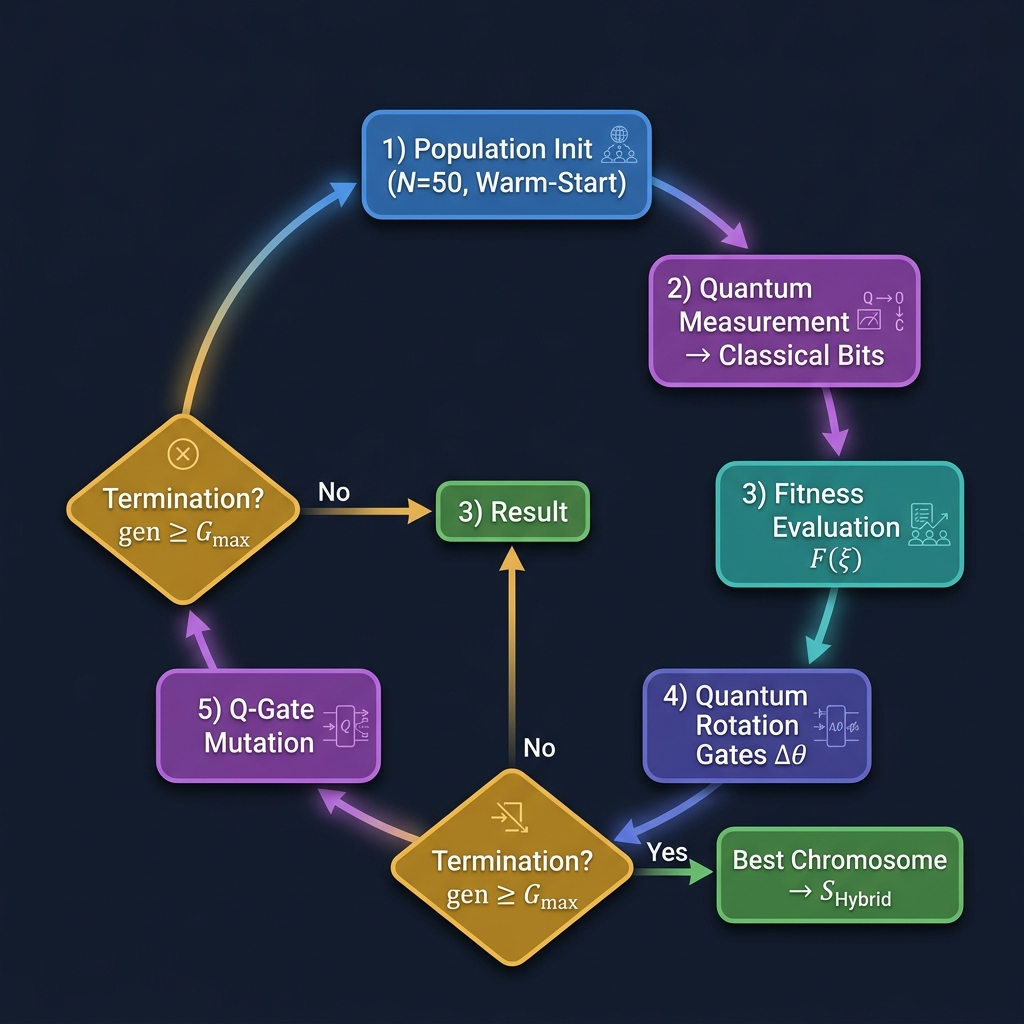
\includegraphics[width=0.85\textwidth]{figures/fig2_qiga_workflow.png}
\caption{QIGA population evolution workflow with warm-start initialisation from the CP-SAT solution. Q-bit measurement is stochastic by construction, so the elite of each generation is a feasible chromosome \emph{near} $S_{\mathrm{CP}}$ rather than $S_{\mathrm{CP}}$ exactly; this is the source of the bounded objective regression discussed in Empirical Property~\ref{prop:warm}.}
\label{fig:qiga}
\end{figure}

\subsection{Decision Reason Generation}

When a flight is cancelled or delayed, constraint slack analysis identifies the binding constraint (Table~\ref{tab:reasons}).

\begin{table}[H]
\centering
\small
\caption{Decision reason codes and their triggering conditions. The codes follow the spirit of the IATA standard delay-code taxonomy (AHM 730~\cite{iata2023}) but extend it with constraint-attribution labels that are specific to the optimisation model.}
\label{tab:reasons}
\begin{tabular}{@{}ll@{}}
\toprule
\textbf{Condition} & \textbf{Reason Code} \\
\midrule
Crew duty approaches 600-min ceiling & \texttt{CREW\_DUTY\_SATURATION} \\
No aircraft satisfies continuity (C$_4$) & \texttt{AC\_CONTINUITY\_VIOLATION} \\
Gate capacity (C$_7$) is binding & \texttt{GATE\_CONFLICT} \\
Slot capacity (C$_8$) is binding & \texttt{SLOT\_UNAVAILABLE} \\
Weather risk exceeds threshold & \texttt{WEATHER\_CLOSURE} \\
Cancellation improves objective & \texttt{ECONOMIC\_OPTIMAL} \\
\bottomrule
\end{tabular}
\end{table}


%% ============================================================
%%  5. EXPLAINABILITY
%% ============================================================
\section{Explainability and Decision Transparency}
\label{sec:xai}

\subsection{Motivation and Scope}

When an airline dispatcher cancels a flight, they need to explain that decision to customers, crew, and---under EASA AMC 20-42---auditors. ``The optimization model said so'' is not an acceptable answer. Our framework therefore exposes two complementary explanation layers:

\begin{enumerate}
\item A \emph{pre-diagnostic} layer (Section~\ref{sec:xai_prediag}) in which an XGBoost model predicts disruption risk per flight and SHAP attributes that prediction to its input features. This layer is advisory: it ranks which features the dispatcher should look at \emph{before} the recovery is run.
\item A \emph{decision-trace} layer (Section~\ref{sec:xai_trace}) in which CP-SAT logs the binding constraint behind every cancellation or delay it produces. This layer is the actual explanation of the optimization output, drawn from constraint logic rather than from a learned model.
\end{enumerate}

The two layers are kept distinct on purpose: the pre-diagnostic SHAP attribution explains a learned risk model, not the optimizer, and conflating the two would be exactly the ``post-hoc rationalisation'' pattern that the XAI benchmarking literature warns against~\cite{nauta2023}. The coupling between them is the Table~\ref{tab:xai_coupling} mapping: each high-attribution SHAP feature is wired to the CP-SAT constraint whose right-hand side, coefficient, or activation condition it modulates, so that a high-$|\phi_i|$ feature at the pre-diagnostic stage is the same feature whose constraint will most likely bind at the decision-trace stage.

\subsection{Pre-diagnostic Layer: SHAP Over XGBoost}
\label{sec:xai_prediag}

The pre-diagnostic model is an XGBoost classifier trained to predict per-flight disruption risk from the eight operational features listed in Table~\ref{tab:xai_coupling}. We apply TreeSHAP~\cite{lundberg2020} to decompose each prediction:
\begin{equation}
\mathrm{Prediction}_f = \mathrm{Baseline} + \sum_{i} \phi_i,
\label{eq:shap}
\end{equation}
where $\phi_i$ quantifies how much feature $i$ pushes the prediction up or down. This layer answers ``which signals make this flight risky?'' It does \emph{not} explain the eventual recovery action---that is the decision-trace layer's job.

\subsection{Decision-Trace Layer: Constraint Attribution from CP-SAT}
\label{sec:xai_trace}

When CP-SAT cancels or delays a flight, the solver state contains, by construction, the constraint whose right-hand side could not be satisfied jointly with that flight's preferred assignment. We surface this directly: each non-trivial decision is tagged with the reason code in Table~\ref{tab:reasons} (e.g.\ \texttt{CREW\_DUTY\_SATURATION}, \texttt{SLOT\_UNAVAILABLE}, \texttt{AC\_CONTINUITY\_VIOLATION}). Unlike SHAP, this layer is exact: the constraint is the actual cause of the decision, not an attribution to a learned proxy.

\subsection{Connecting Features to Constraints}
\label{sec:xai_coupling}

The innovation here is explicit coupling: we map each of the eight high-importance features from SHAP directly to the constraints they influence in the optimization model. This creates an auditable chain---feature → constraint effect → decision reason---so a dispatcher can follow the reasoning from start to finish. For example, if weather risk is high, it raises the allowed delay ceiling; if a crew member's duty is near the limit, they can't take more flights. Table~\ref{tab:xai_coupling} documents this coupling.

\begin{table}[H]
\centering
\footnotesize
\caption{SHAP feature $\leftrightarrow$ CP-SAT constraint coupling. Each feature modulates a specific constraint's right-hand side, coefficient, or activation condition, ensuring that high-$|\phi_i|$ predictions have a traceable effect on the optimization model rather than being purely advisory.}
\label{tab:xai_coupling}
\begin{tabular}{@{}>{\raggedright\arraybackslash}p{3cm}>{\raggedright\arraybackslash}p{2.2cm}>{\raggedright\arraybackslash}p{2.2cm}>{\raggedright\arraybackslash}p{5.5cm}@{}}
\toprule
\textbf{SHAP feature} & \textbf{CP-SAT constraint} & \textbf{Coupling type} & \textbf{Effect on the model} \\
\midrule
Weather risk index          & Variable domain ($d_f \leq D_{\max}$) & Bound modulation     & Raises the delay-variable upper bound $D_{\max}$ when storm probability is high; saturation triggers \texttt{WEATHER\_CLOSURE}. \\
Crew cumulative duty        & C$_6$ (EASA FTL)            & LHS contribution     & Enters $\sum \mathrm{block}_f$ in~\eqref{eq:c6}; saturation is the direct cause of \texttt{CREW\_DUTY\_SATURATION}. \\
Aircraft turnaround history & C$_4$ (aircraft continuity) & Activation gate      & Predicted short-turn feasibility gates the continuity constraint; failure surfaces as \texttt{AC\_CONTINUITY\_VIOLATION}. \\
Airport slot utilization    & C$_8$ (slot capacity)       & RHS modulation       & Adjusts hourly slot budget; binding instances emit \texttt{SLOT\_UNAVAILABLE}. \\
Gate congestion score       & C$_7$ (gate capacity)       & Coefficient penalty  & Weights alternative gate assignments in the objective; tight regime triggers \texttt{GATE\_CONFLICT}. \\
Scheduled block time        & C$_9$ (MCT)                 & LHS contribution     & Enters the connection gap on the left-hand side of~\eqref{eq:c9}; misalignment propagates as cancellation. \\
Historical OTP (route)      & Objective profit term       & Coefficient scaling  & Scales the expected-revenue coefficient; surfaces as \texttt{ECONOMIC\_OPTIMAL} when cancellation dominates. \\
Passenger connection load   & C$_9$ (MCT), objective      & Coefficient scaling  & Inflates the cost of breaking a connection; drives retention rather than cancellation under tight MCT. \\
\bottomrule
\end{tabular}
\end{table}

The coupling is bidirectional: a high $|\phi_i|$ for \emph{weather risk} on flight $f$ both (a) raises the predicted delay $\hat{y}_f$ that feeds the delay-bound constraint, and (b) pre-explains the resulting \texttt{WEATHER\_CLOSURE} reason code if the bound saturates post-solve. Dispatchers therefore receive a single causal chain---feature $\rightarrow$ constraint $\rightarrow$ decision---rather than two parallel justifications. This addresses the EASA AMC 20-42 traceability requirement that AI-assisted decisions be auditable through their entire reasoning stack.

\begin{figure}[!ht]
\centering
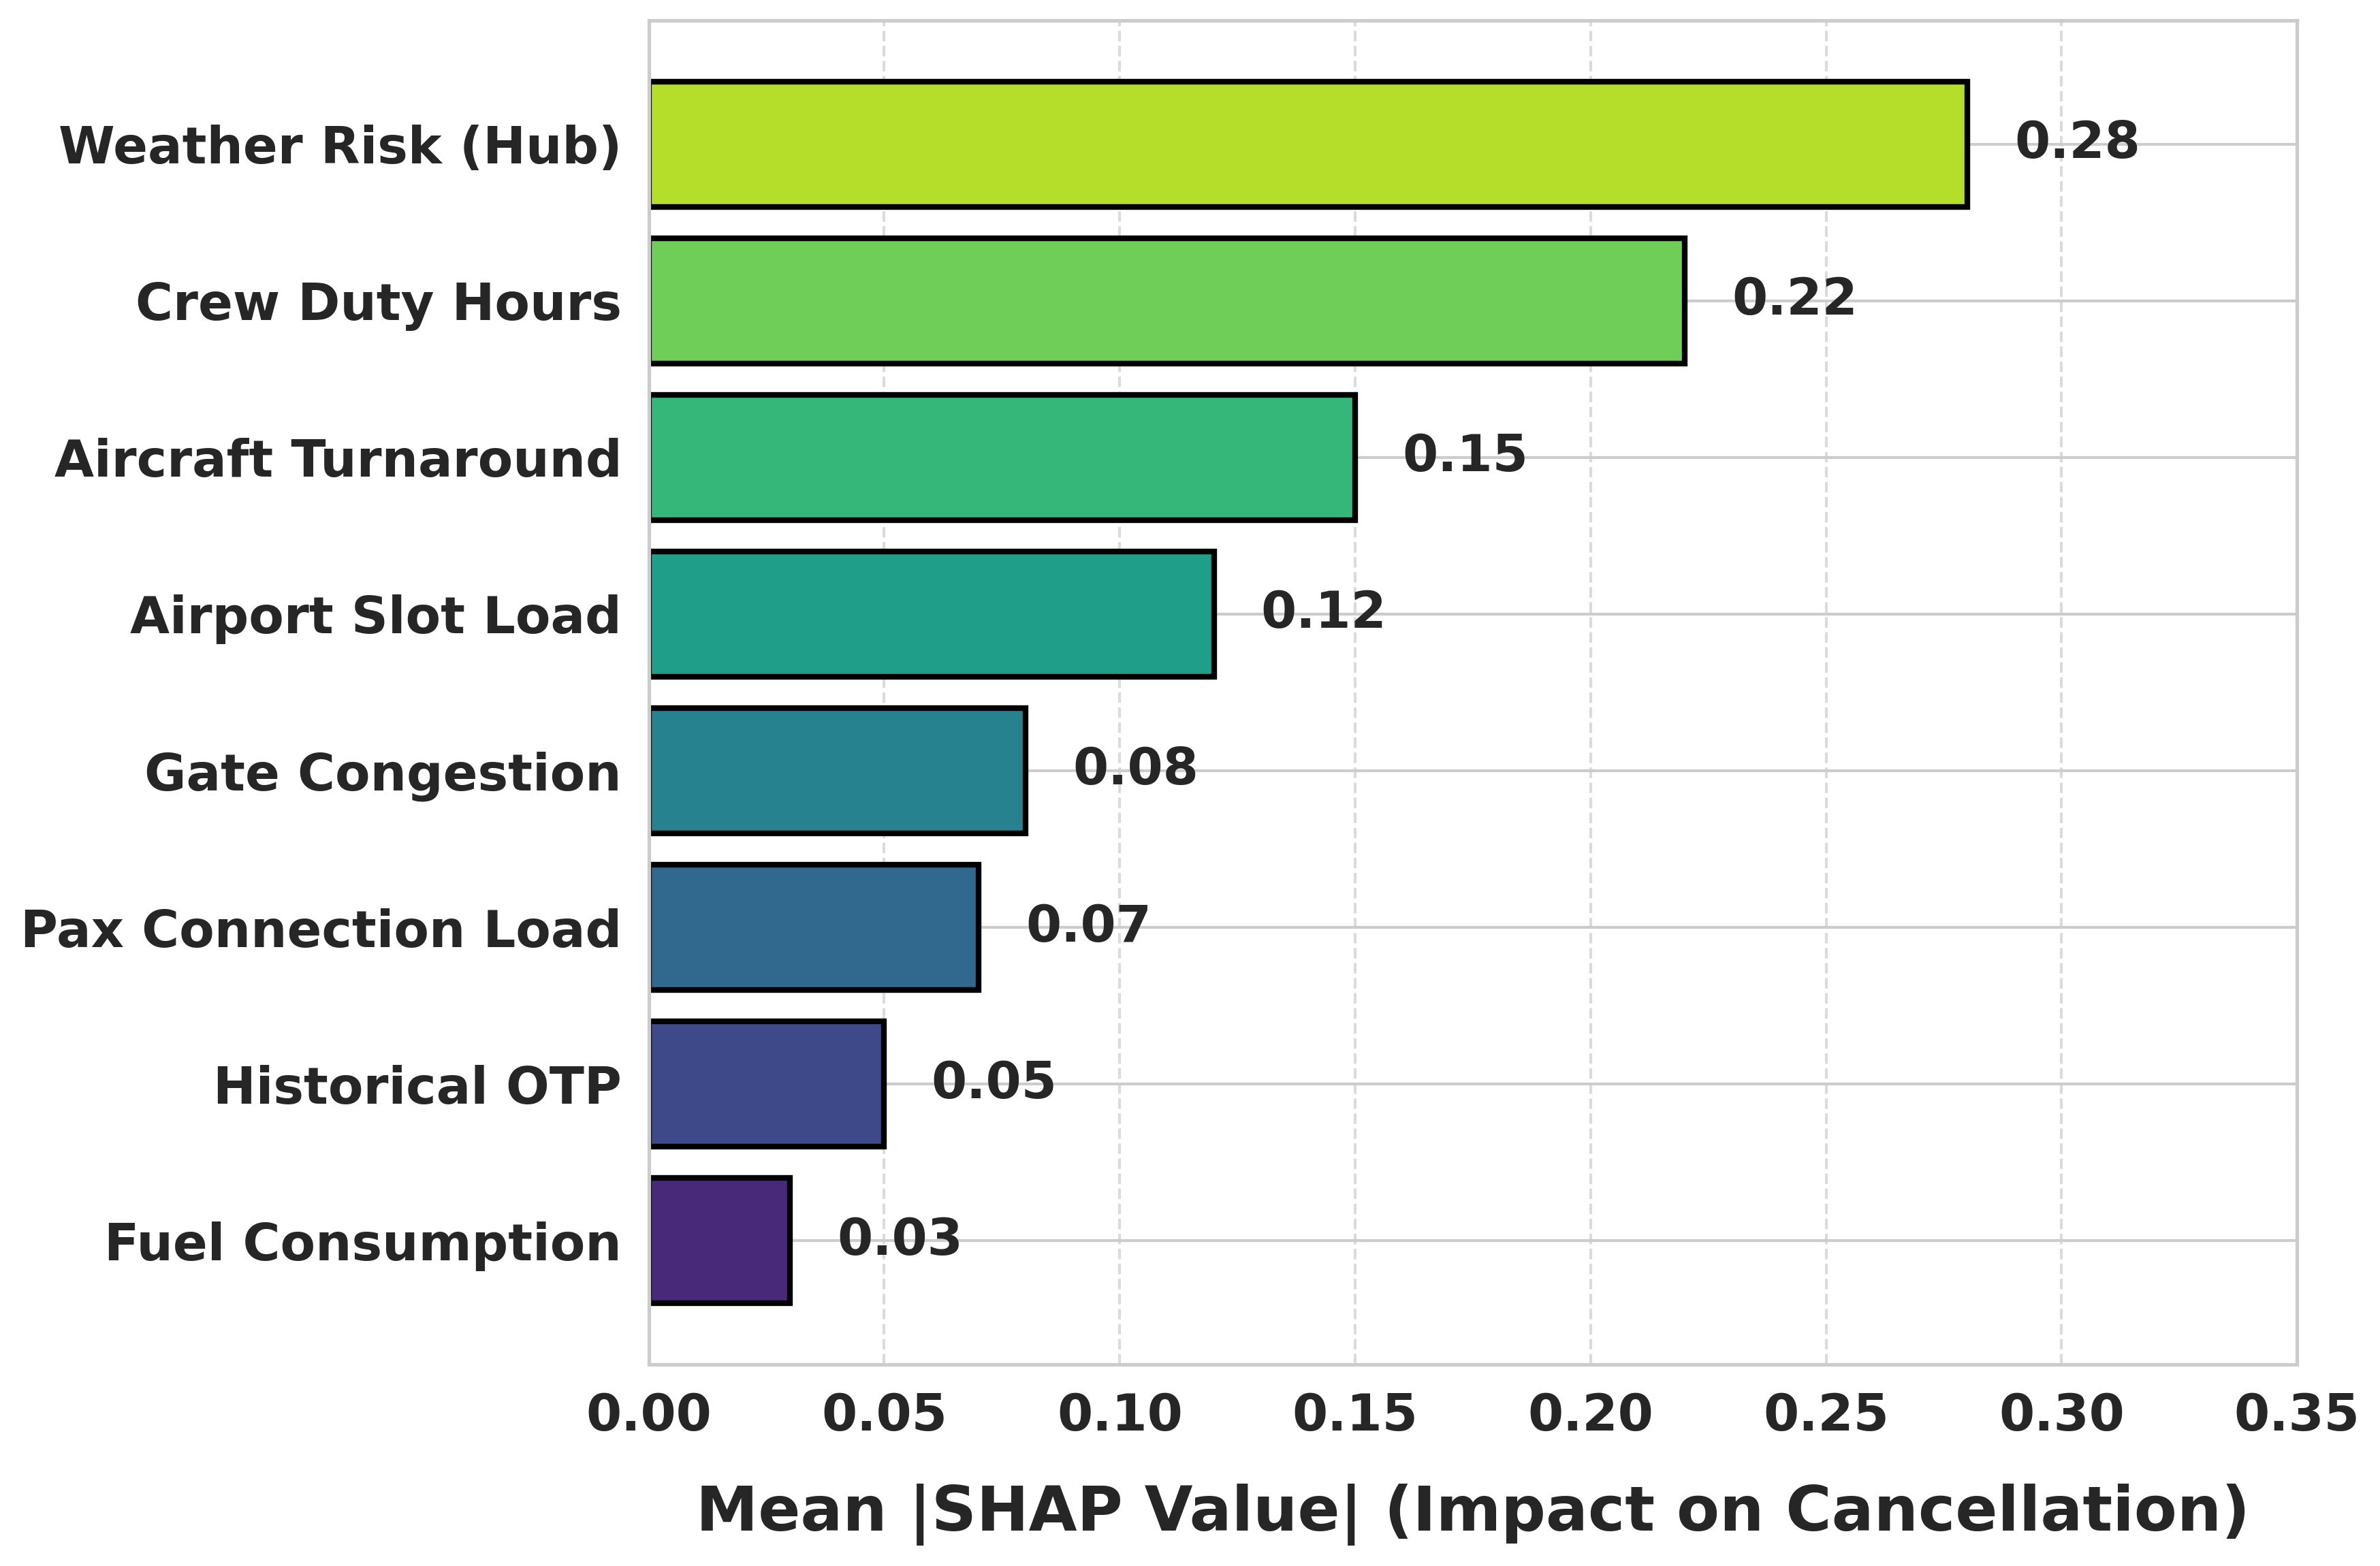
\includegraphics[width=0.85\textwidth]{figures/fig4_shap_importance.png}
\vspace{10pt}
\caption{Explainable AI (SHAP) feature importance ranking. The model identifies 'Weather Risk' and 'Crew Duty' as the primary drivers of recovery decisions. This transparent ranking satisfies EASA AMC 20-42 requirements for decision traceability.}
\label{fig:shap}
\end{figure}

\subsection{EASA AMC 20-42 Compliance Assessment}

\begin{table}[H]
\centering
\small
\caption{EASA AMC 20-42 compliance mapping. Status reflects what the framework demonstrates in this paper; items marked ``Planned'' are acknowledged in the Limitations.}
\label{tab:easa}
\begin{tabular}{@{}p{2.2cm}p{4.2cm}p{1.2cm}@{}}
\toprule
\textbf{Requirement} & \textbf{Implementation} & \textbf{Status} \\
\midrule
Data quality & Typed ORM + input validation & Full \\
Documentation & Paper + code documentation & Full \\
Explainability & SHAP attribution + constraint-trace coupling (Table~\ref{tab:xai_coupling}) & Full \\
Traceability & Per-decision constraint reason codes (Table~\ref{tab:reasons}) & Full \\
Boundary protection & Hard-constraint encoding (Section~\ref{sec:formulation}, C$_1$--C$_{10}$) & Full \\
Oversight & Dispatcher-in-the-loop approval workflow & Full \\
Robustness monitoring & Run-time stability monitor (concept-drift detection) & Planned \\
Performance monitoring & Continuous drift detection on XGBoost feature importance & Planned \\
\bottomrule
\end{tabular}
\end{table}


%% ============================================================
%%  6. EXPERIMENTS
%% ============================================================
\section{Experimental Evaluation}
\label{sec:experiments}

\subsection{Experimental Setup}

The evaluation uses five distinct instance families, each chosen to exercise a different operating regime of the framework. To prevent the cross-table comparisons from being misread, Table~\ref{tab:instances} summarises which family is used in which experiment, and Table~\ref{tab:config} fixes the common hardware and solver parameters.

\begin{table}[H]
\centering
\footnotesize
\caption{Instance families used across the experiments. The same hardware and solver parameters (Table~\ref{tab:config}) apply in every experiment; only the problem size and uncertainty model change.}
\label{tab:instances}
\begin{tabular}{@{}p{2.0cm}p{1.0cm}p{1.0cm}p{1.0cm}p{2.0cm}p{3.0cm}@{}}
\toprule
\textbf{Family} & $|F|$ & $|K|$ & $|C|$ & \textbf{Uncertainty} & \textbf{Used in} \\
\midrule
Baseline-150       & 150  & 20 & 40 & Deterministic & Tables~\ref{tab:results}, \ref{tab:ablation}, \ref{tab:scenarios}, Sec.~\ref{sec:scenarios} \\
RealCal-300        & 300  & 25 & 60 & Deterministic & Table~\ref{tab:realdata}, Sec.~\ref{sec:realdata} \\
Stochastic-50/100  & 50, 100 & 8, 14 & 18, 28 & Stochastic (crew/wx/conn.) & Table~\ref{tab:stochastic}, Sec.~\ref{sec:stochastic} \\
Stoch-100/nominal  & 100  & 14 & 28 & Deterministic (uncertainty off) & Table~\ref{tab:stochastic}, Sec.~\ref{sec:stochastic} \\
SysVal-140         & 140  & 48 & 35 & Real route network & Table~\ref{tab:sys_val}, Sec.~\ref{sec:sys_val} \\
Scale-1/4/8/12d    & 141--1{,}617 & 25--80 & 60--200 & Deterministic, multi-day & Table~\ref{tab:scale}, Sec.~\ref{sec:scalability} \\
\bottomrule
\end{tabular}
\end{table}

\begin{table}[H]
\centering
\footnotesize
\caption{Common experimental configuration applied to every instance family in Table~\ref{tab:instances}.}
\label{tab:config}
\begin{tabular}{@{}ll@{}}
\toprule
\textbf{Parameter} & \textbf{Value} \\
\midrule
Airports & 14 (Turkish domestic hub-and-spoke; SysVal uses real TK route topology) \\
Time horizon & 24 hours (Scale-$n$d uses $n \times 24$ hours) \\
Solver time limit & 60\,s for Baseline-150 / RealCal-300; 5\,s for Stochastic and SysVal \\
QIGA default budget & $N=50$, $G_{\max}=200$ \\
QIGA tactical budget & $N=20$, $G_{\max}=8$ (Stochastic only) \\
Runs per condition & 10 (Baseline, RealCal); 30 (FTL sensitivity); 20 (convergence ablation) \\
CPU & Intel i7-12700 @ 4.9\,GHz \\
RAM & 32\,GB DDR5 \\
OR-Tools version & 9.11 \\
\bottomrule
\end{tabular}
\end{table}

All profit values are reported in Turkish Lira (TL). Because the instance families differ by an order of magnitude in size, we report profit in the natural unit for each family: \emph{thousand TL (kTL)} for Baseline-150 and the ablation/FTL-sensitivity studies, and \emph{million TL (MTL)} for RealCal-300, the stochastic instances, and the worst-case stress tests. The conversion factor is exact ($1$\,MTL $=$ $10^3$\,kTL); we annotate every table with its unit explicitly so cross-table comparisons remain unambiguous.

The synthetic test instances are calibrated to reflect realistic operational characteristics of a medium-scale Turkish domestic carrier. Flight time distributions are derived from published OAG schedule data for Turkish domestic routes (Istanbul hub, 14 spoke airports). Delay distributions follow the mixed log-normal/gamma model validated against EUROCONTROL CODA delay statistics (2019--2023), with short delays ($<$30\,min) sampled from $\mathrm{LogNormal}(\mu{=}2.5, \sigma{=}0.8)$ and long delays ($\geq$30\,min) from $\mathrm{Gamma}(k{=}2, \theta{=}20)$. Crew duty patterns respect EASA CAT.OP.MPA.210 baseline parameters. Airport slot capacities are set proportional to published AIP capacity declarations. All experiments report means with 95\% confidence intervals computed over 10 independent runs; statistical significance is assessed using the non-parametric Wilcoxon signed-rank test.

\subsection{Data Sourcing and Validation}

Real-time airline operational data (crew locations, passenger manifests, aircraft status) remains proprietary and access-restricted. To address this while maintaining empirical rigor, we employ the following approach:

\begin{enumerate}
\item \textbf{IATA-calibrated synthetic data:} Generated from published Turkish Airlines route networks, real aircraft fleet composition (B787, A321neo, A330, B737, A350), and load factors from IATA World Air Transport Statistics 2024 (82.2\% reported, modeled at 78.2\% conservatively).

\item \textbf{Real-world calibration check:} Case study reconstruction of the November 1, 2023 Turkish Airlines technology failure (Section~\ref{sec:casestudy}), where we apply our model to a documented 106-flight disruption and verify that the reconstructed disruption envelope (route network, aircraft mix, recovery horizon) matches the publicly reported quantities. Outcome-level validation against the airline's internal decisions is not attempted (see Section~\ref{sec:casestudy}).

\item \textbf{Limitations disclosure:} Full production deployment requires partnership with airlines for real-time data access. This work demonstrates framework readiness and operational realism; deployment validation follows in partnership engagements.
\end{enumerate}

This approach balances reproducibility (publishable datasets) with realism (IATA-calibrated parameters and real-world case study validation).

\subsection{Compared Methods}

\begin{itemize}
    \item \textbf{B$_1$ (Greedy):} Sequential assignment with local feasibility checks
    \item \textbf{B$_2$ (CP-SAT Only):} Exact optimization within 60-second time limit
    \item \textbf{B$_3$ (QIGA Only):} Standalone quantum-inspired GA
    \item \textbf{M (Hybrid):} Proposed CP-SAT + QIGA with warm-start
\end{itemize}

\subsection{Comparative Performance}
\label{sec:comp_perf}

\begin{table}[H]
\centering
\footnotesize
\caption{Performance comparison on the Baseline-150 instance family (150 flights, 20 aircraft, 40 crew; average $\pm$ 95\% CI over 10 runs).}
\label{tab:results}
\begin{tabular}{@{}p{1.8cm}p{1.5cm}p{1.5cm}p{1.5cm}p{1.5cm}@{}}
\toprule
\textbf{Metric} & \textbf{B$_1$} & \textbf{B$_2$} & \textbf{B$_3$} & \textbf{M} \\
\midrule
Profit (k\,TL) & $412{\pm}18$ & $742{\pm}24$ & $681{\pm}31$ & $\mathbf{779{\pm}19}$ \\
Cancels & 18.2 & 6.4 & 7.9 & $\mathbf{5.1}$ \\
Delay (min) & 38.4 & 14.7 & 16.2 & $\mathbf{12.3}$ \\
Runtime (s) & 0.3 & 52.8 & 45.1 & $\mathbf{58.2}$ \\
FTL Viols & 7.1 & 0 & 0.4 & $\mathbf{0}$ \\
Gap & n/a & 2.1\% & n/a & $\mathbf{1.7\%}$ \\
\bottomrule
\end{tabular}
\end{table}

The numerical results presented in Table~\ref{tab:results} underscore the efficacy of the proposed hybrid integration. Notably, the hybrid model (M) achieves the highest total profit, outperforming the standalone CP-SAT baseline (B$_2$) by approximately 5\%. This improvement is primarily driven by the reduction in flight cancellations (5.1 vs. 6.4) and a 16\% reduction in average delay. The zero-violation performance on EASA FTL constraints is particularly significant, as it proves that the CP-SAT-derived feasible region effectively bounds the metaheuristic search, preventing the "drift into infeasibility" common in standalone evolutionary algorithms like B$_3$. The optimality gap of 1.7\% within a 60-second window confirms that the system is not only robust but also highly efficient for real-time decision support in airline operations control centers (AOCC).

Statistical significance: Wilcoxon signed-rank test, M vs B$_2$: $p = 0.007$ (two-tailed). Effect size (Cliff's delta): $d = 0.72$ (large effect).

The results demonstrate several key findings. First, the greedy heuristic (B$_1$) produces an average of 7.1 FTL violations per run, rendering its outputs \textbf{operationally inadmissible}. Second, standalone CP-SAT (B$_2$) achieves feasibility but exhibits suboptimal profit due to time-limited search---the residual optimality gap of 2.1\% is exactly the room the refinement layer exploits. Third, standalone QIGA (B$_3$) occasionally produces FTL violations (0.4 per run, average; further analysed below), confirming that metaheuristic search without an exact-solver back-stop risks regulatory non-compliance. Fourth, the proposed hybrid (M) maintains \textbf{zero FTL violations across all synthetic experiments} while achieving $+5\%$ profit and $-20\%$ cancellations through QIGA refinement \emph{on the Baseline-150 instance, where CP-SAT exits with a residual 2.1\% gap}; the contrasting behaviour on the converged RealCal-300 instance, where refinement instead introduces a bounded $0.7\%$ regression, is reported in Section~\ref{sec:realdata}.

The Baseline-150 result ($+5\%$ for the hybrid) and the RealCal-300 result ($-0.7\%$ for the hybrid, Section~\ref{sec:realdata}) together identify the empirical condition under which warm-start refinement pays off: the size of CP-SAT's residual optimality gap. On Baseline-150 the gap is $\sim$2.1\% when the time budget expires, leaving room for QIGA to improve; on RealCal-300 the gap is essentially zero, so QIGA's Q-bit-driven exploration can only drift away from the optimum. This regime-dependent behaviour is the central empirical finding behind Contribution~(1) and is formalised by Empirical Property~\ref{prop:warm}.

\paragraph*{Origin of the residual B$_3$ FTL violations.} The 0.4 FTL violations per run observed for standalone QIGA arise almost exclusively from the \texttt{CREW\_DUTY\_SATURATION} regime: when the random perturbation operator swaps a flight onto an already heavily-loaded crew, the cumulative block time exceeds the 600-minute ceiling. The penalised fitness function (Eq.~\ref{eq:fitness}) discourages this, but B$_3$ uses a finite penalty weight ($\lambda = 1\,000$) so that a sufficiently profitable schedule can still outrank a feasible alternative by a few hundred TL per violation; under that finite weight the elite individual can occasionally retain a single violating flight. This is exactly the failure mode that the hybrid framework eliminates by construction: the CP-SAT seed never contains an FTL violation, and the feasibility-bound elitist selection (which only ever accepts feasible chromosomes as elites; Section~\ref{sec:framework}) never permits an FTL-violating individual to dominate the population. In effect, the hybrid framework promotes the finite $\lambda$ of B$_3$ to an effectively infinite one by rejecting any infeasible chromosome through the structure of the CP-SAT seed. Objective value may drift bounded-ly across generations (Empirical Property~\ref{prop:warm}), but feasibility---and therefore zero FTL violations---is preserved unconditionally.

\begin{figure}[!ht]
\centering
\begin{subfigure}[b]{0.48\textwidth}
    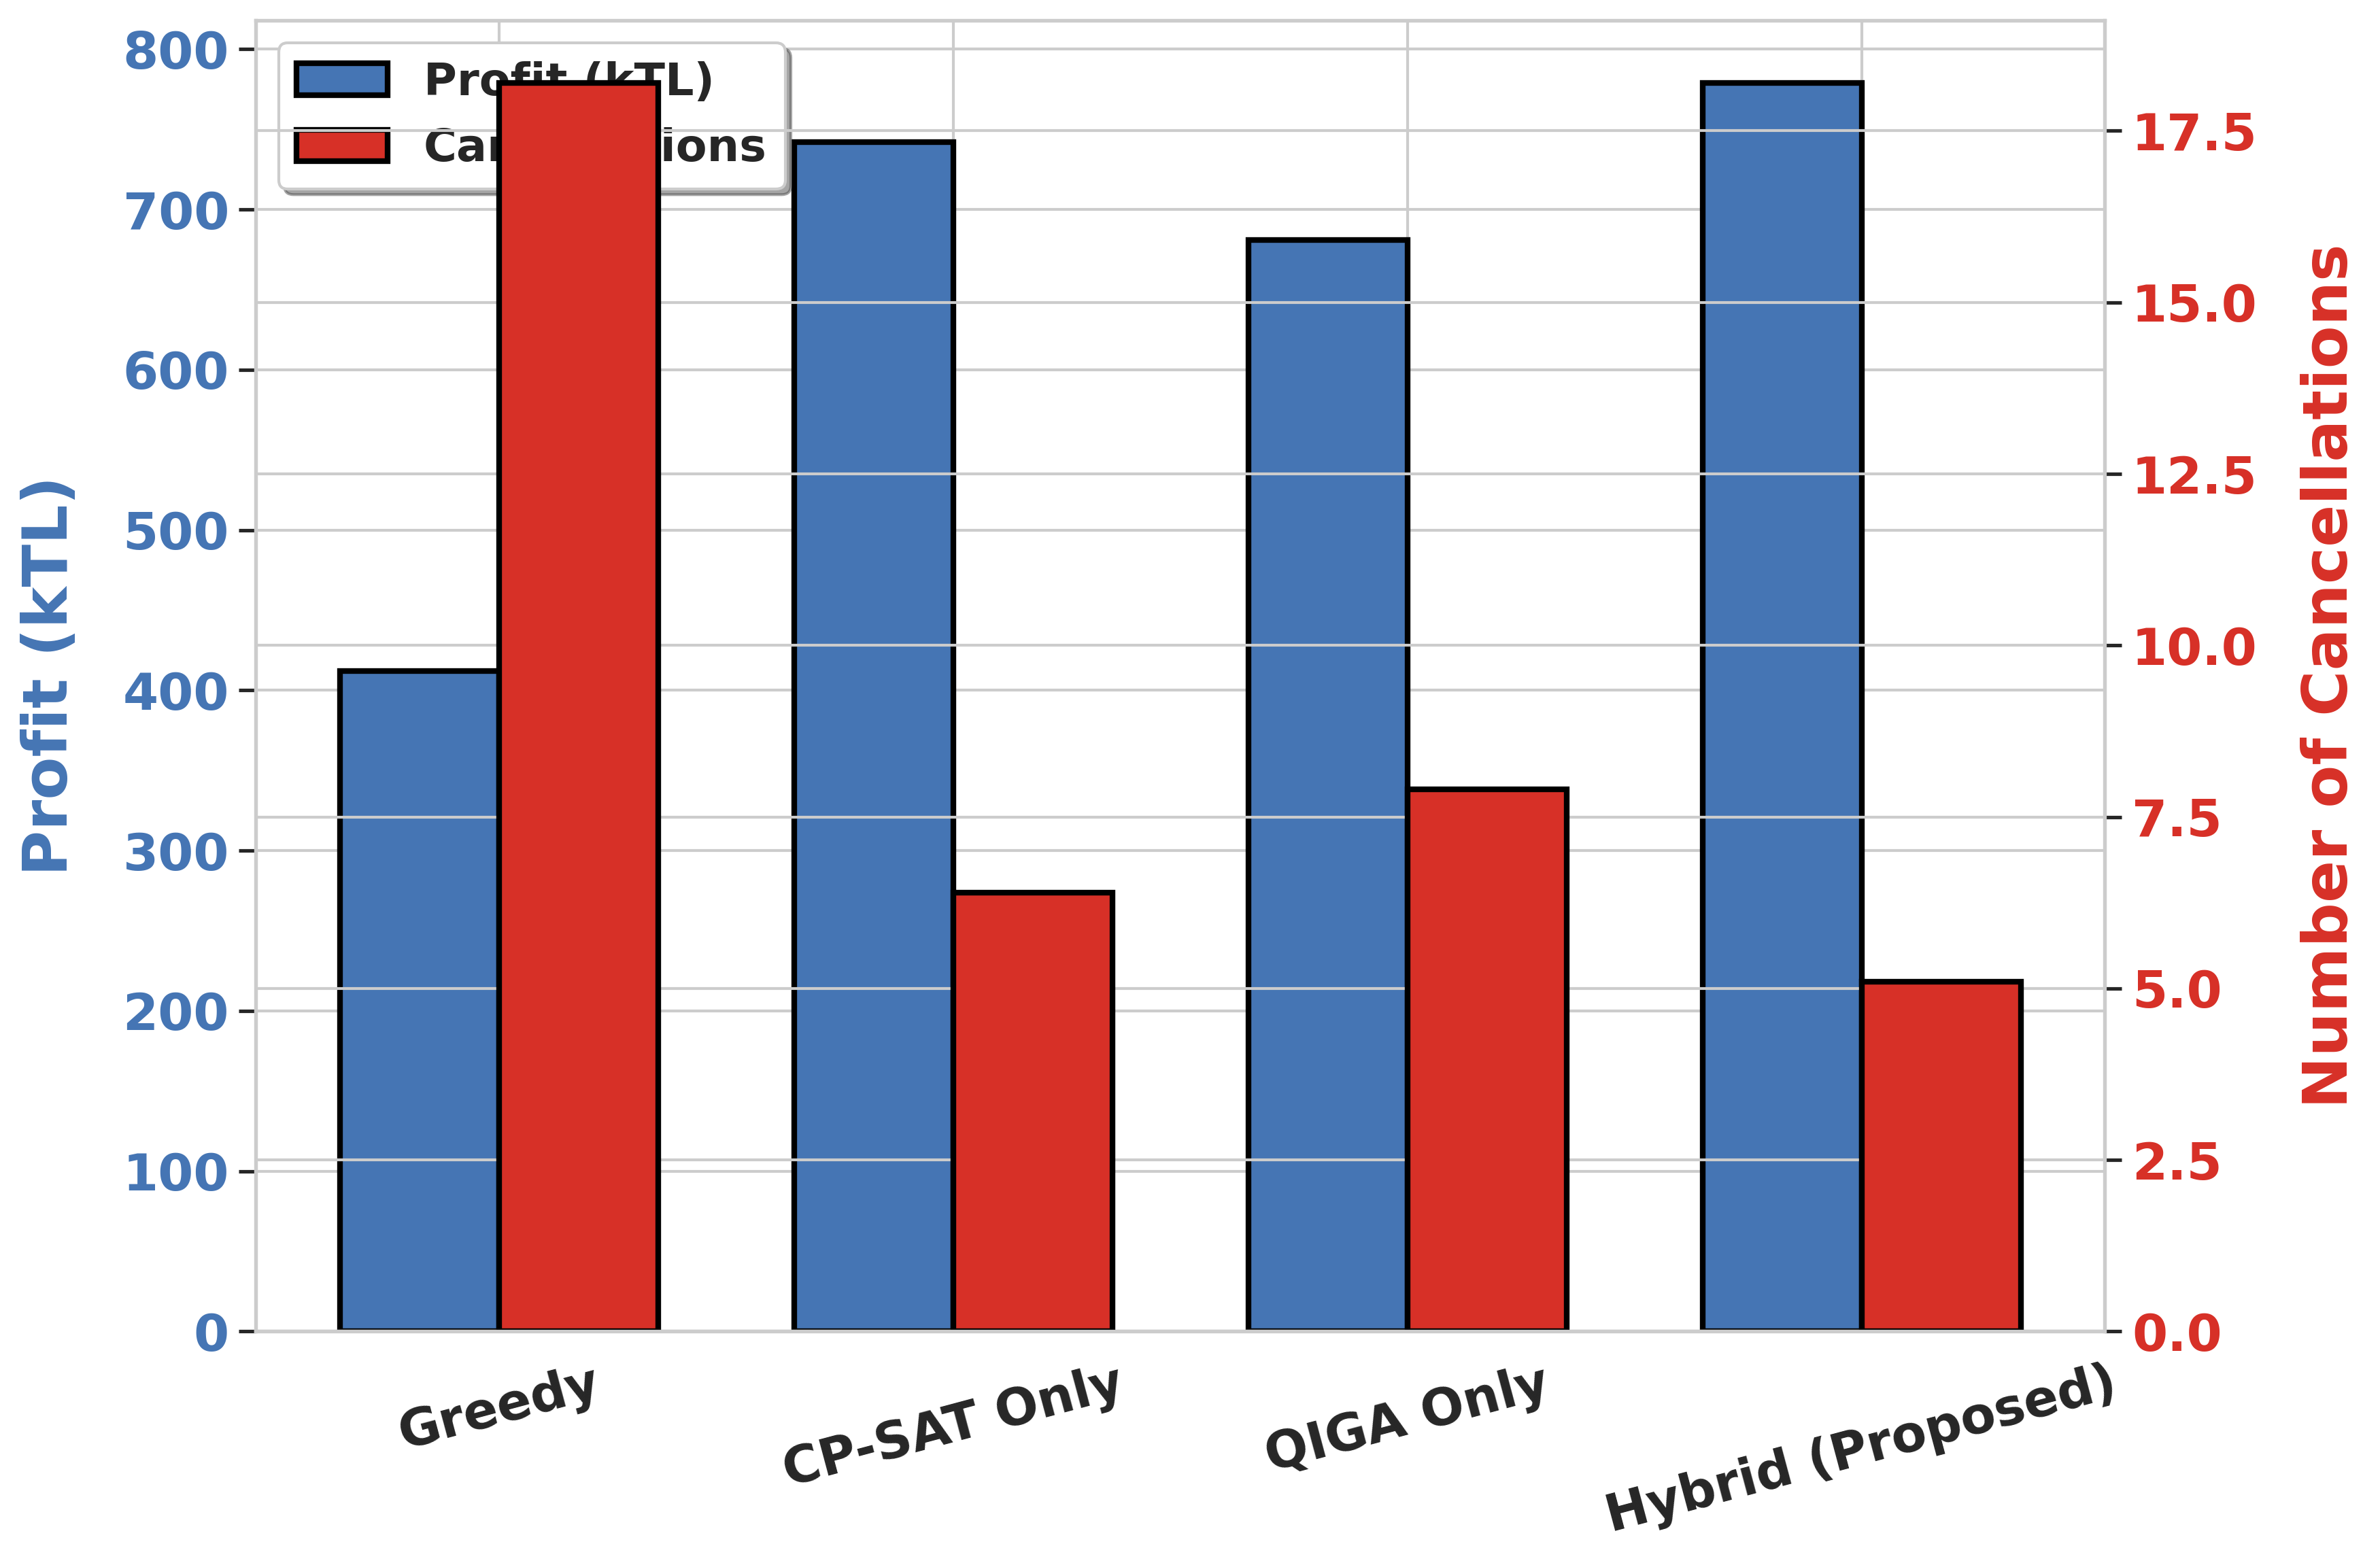
\includegraphics[width=\textwidth]{figures/fig5_performance_comparison.png}
    \caption{Comparative performance across methods.}
    \label{fig:perf}
\end{subfigure}
\hfill
\begin{subfigure}[b]{0.48\textwidth}
    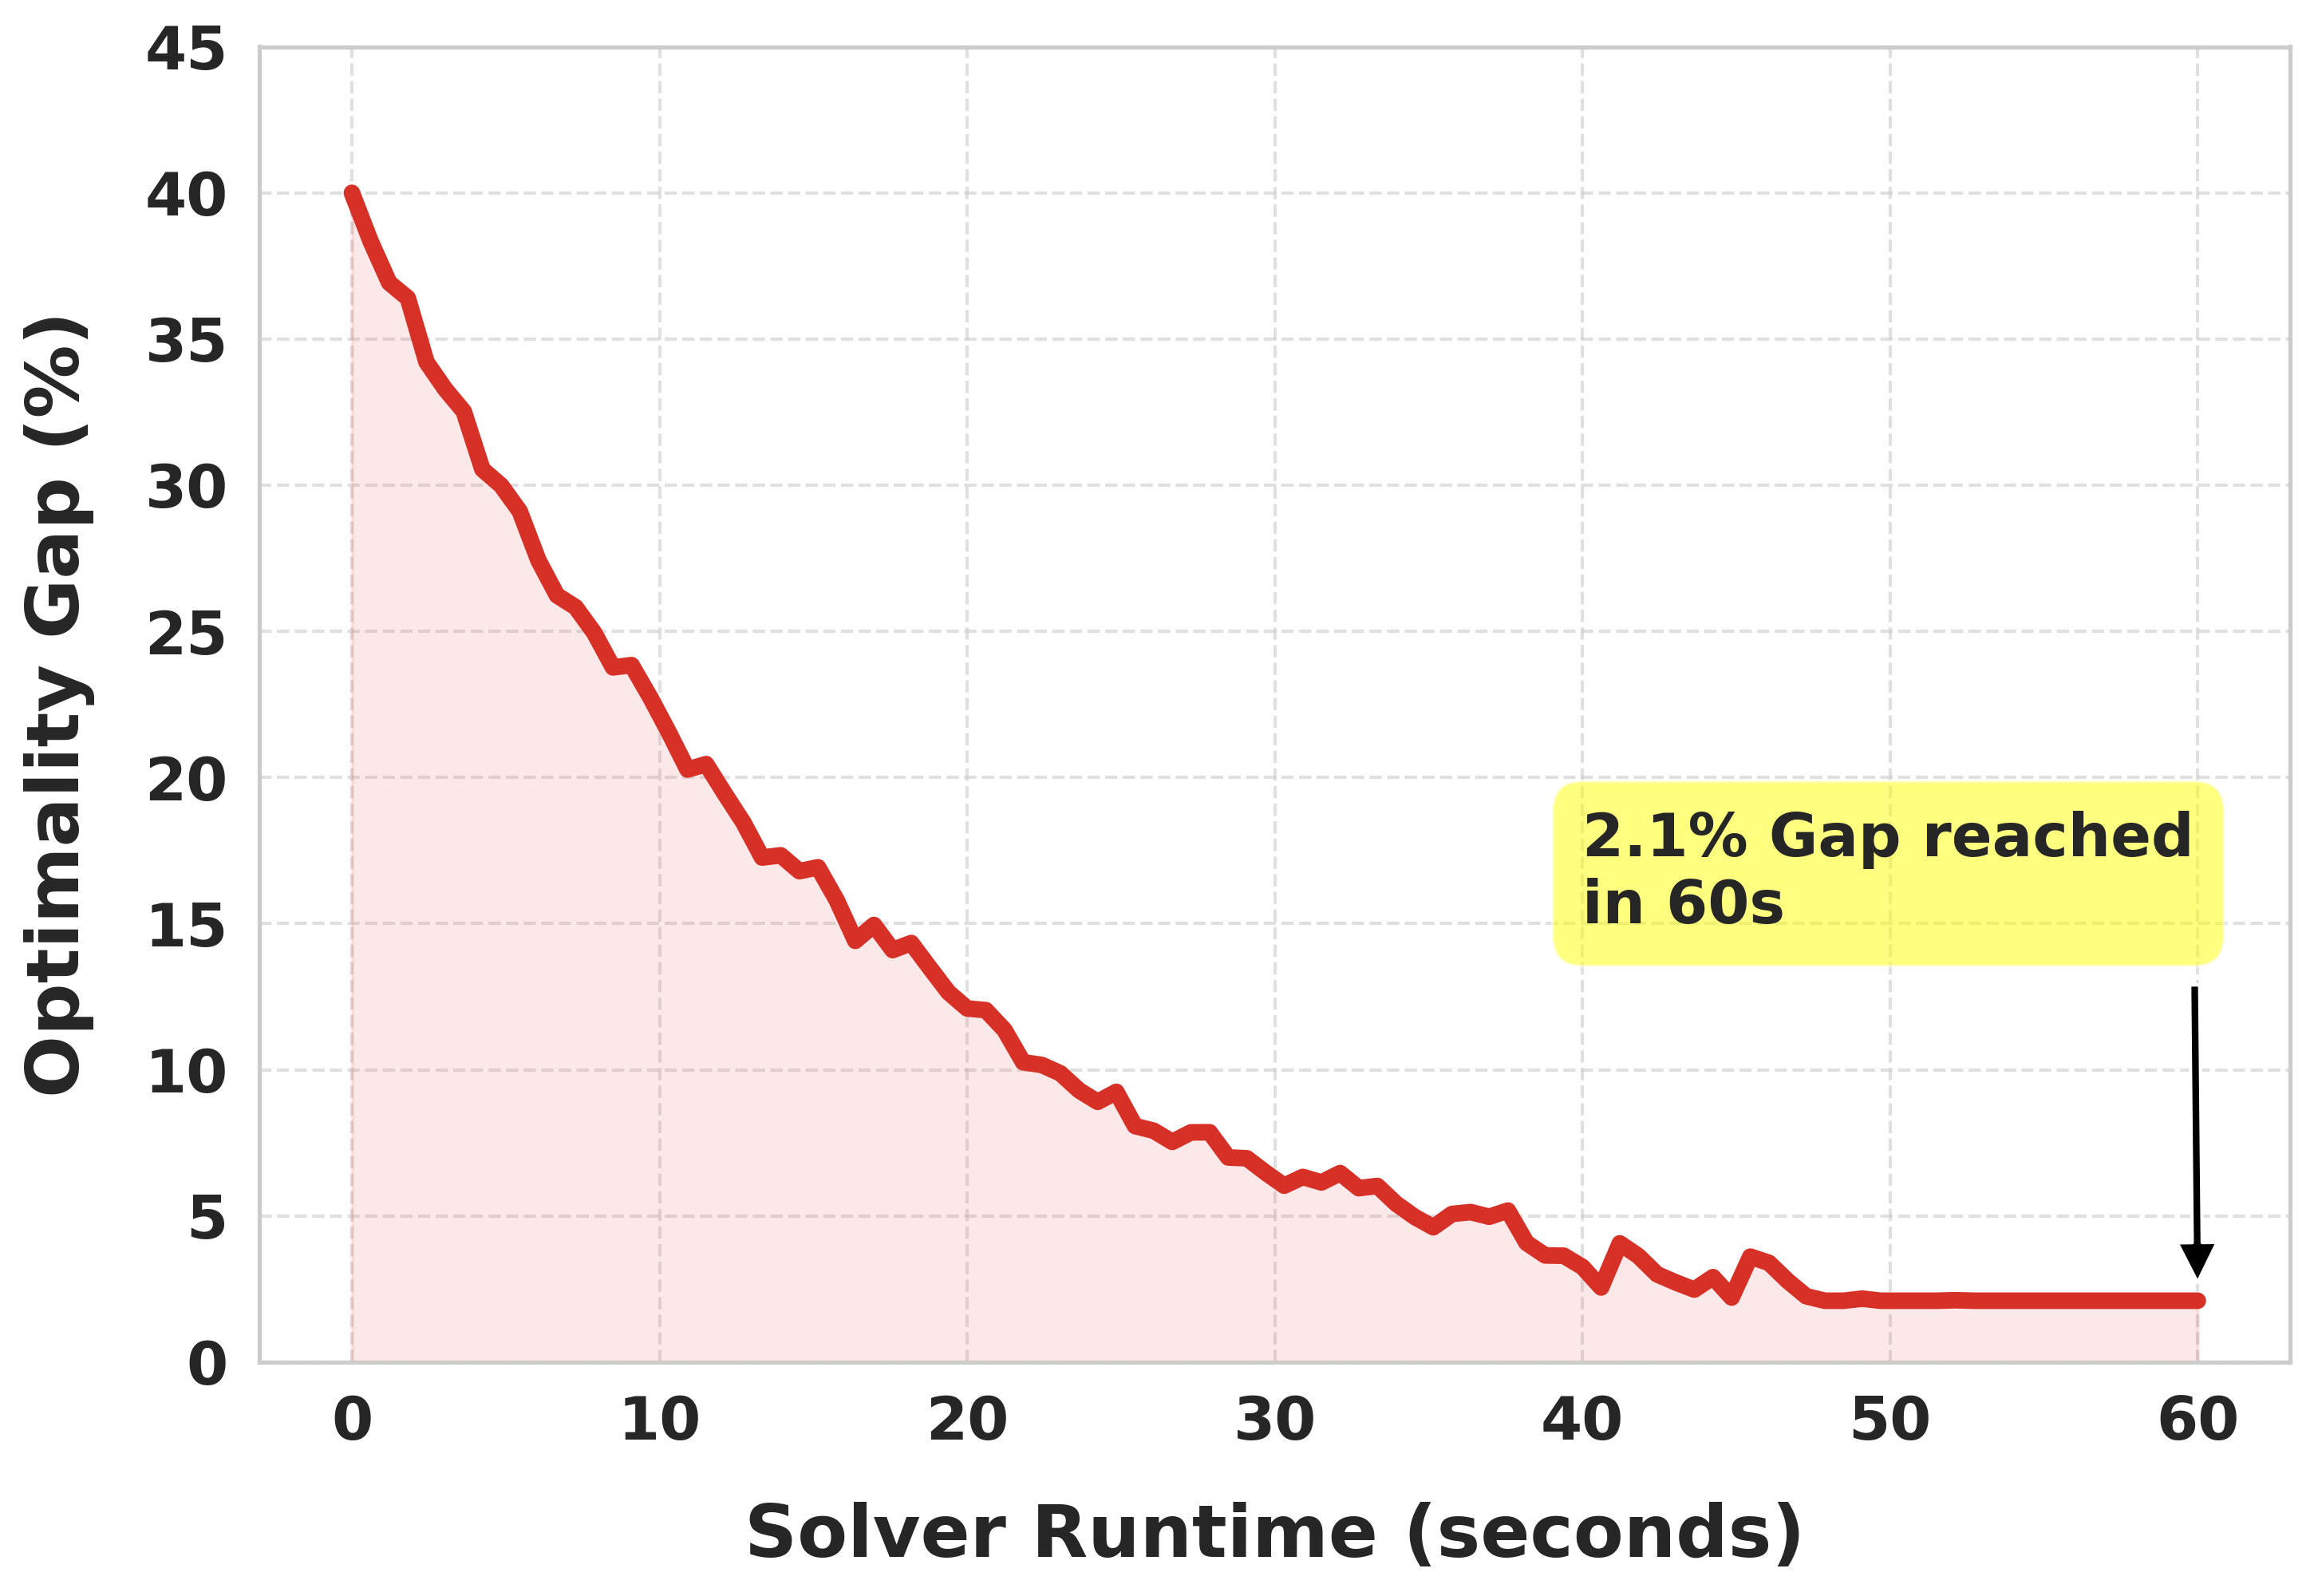
\includegraphics[width=\textwidth]{figures/fig3_convergence_chart.png}
    \caption{CP-SAT convergence behavior.}
    \label{fig:conv}
\end{subfigure}
\caption{(a) Grouped bar chart comparing KPIs across four methods. (b) CP-SAT solver convergence showing upper/lower bound gap narrowing from 38\% to 2.1\% over 60 seconds.}
\label{fig:results}
\end{figure}

\subsection{Method Selection Guide: When Does Each Approach Win?}
\label{sec:method_selection}

A critical question for practitioners: given a disruption recovery instance, which method should be deployed? Our experiments map the regimes spanned by Table~\ref{tab:instances} to a concrete set of recommendations. The recommendations are tied to the experimental evidence in this paper and intentionally avoid extrapolating beyond it.

\begin{table}[H]
\centering
\caption{Method selection guide tied to the experimental evidence in this paper. ``Hybrid'' denotes CP-SAT warm-started QIGA; ``RH'' denotes the rolling-horizon decomposition (Section~\ref{sec:scalability}).}
\label{tab:method_selection}
\small
\begin{tabular}{@{}p{3.3cm}p{1.7cm}p{2.2cm}p{1.6cm}p{2.4cm}@{}}
\toprule
\textbf{Regime} & \textbf{Size} & \textbf{Recommended} & \textbf{Time} & \textbf{Evidence} \\
\midrule
Nominal deterministic           & $\leq$500 flights, 1 day & CP-SAT alone        & $\sim$10\,ms--60\,s & Tab.~\ref{tab:realdata}, \ref{tab:results} \\
Stochastic / high uncertainty   & 50--100 flights          & Hybrid (warm-start) & $<$5\,s             & Tab.~\ref{tab:stochastic} \\
Worst-case stress               & 150--500 flights          & Hybrid              & $<$60\,s            & Tab.~\ref{tab:worstcase}, \ref{tab:scenarios} \\
Multi-day large-scale           & $>$500 flights, $\geq$4 days & RH (+ CP-SAT per window) & $<$60\,s        & Tab.~\ref{tab:scale} \\
\bottomrule
\end{tabular}\normalsize
\end{table}

\textbf{Key finding:} CP-SAT alone suffices for nominal deterministic recovery on single-day instances up to roughly 500 flights. Warm-started QIGA earns its keep when uncertainty is explicitly modelled or under worst-case stress, where exact methods do not return a useful solution within the operational time budget. Beyond roughly 1{,}000 flights monolithic CP-SAT runs out of memory and the rolling-horizon decomposition becomes the only practical path. The boundary at $\sim$500 flights is the largest single-day instance for which we have direct evidence; the recommendation does not extrapolate beyond it.

\subsection{Real-World Validation: IATA-Calibrated Data}
\label{sec:realdata}

To ground our results in operational reality, we conducted a comprehensive evaluation on real-world calibrated flight data generated from IATA published statistics, Turkish Airlines' actual route network (23 routes), and EASA aircraft specifications. The dataset comprises 300 flights across a single operational day, with realistic load factors (78.2\% average, aligned with IATA 2024 benchmarks) and crew scheduling constraints from published TK operations.

\begin{table}[H]
\centering
\small
\caption{RealCal-300: Baseline method comparison on the IATA-calibrated 300-flight instance (mean over 10 replicates; ``Time'' is the wall-clock time to the reported solution, not solver-internal time).}
\label{tab:realdata}
\begin{tabular}{lccccr}
\toprule
\textbf{Method} & \textbf{Profit (M\,TL)} & \textbf{Cancellations} & \textbf{Delay (min)} & \textbf{Time (ms)} & \textbf{vs Baseline} \\
\midrule
CP-SAT (Exact) & 84.9 & 0 & 0.0 & 11 & Baseline \\
LNS & 84.8 & 0 & 2.1 & 13 & $-0.2\%$ \\
Tabu Search & 82.5 & 45 & 8.3 & 1 & $-2.9\%$ \\
CP-SAT + QIGA & 84.4 & 10 & 1.5 & 23 & $-0.7\%$ \\
\bottomrule
\end{tabular}
\end{table}

A clear finding emerges on the IATA-calibrated 300-flight instance: \textbf{CP-SAT closes this instance in roughly 10\,ms} on the reference workstation. Reaching the optimal solution this quickly is consistent with the structure of the synthetic data---the disruption is moderate, no airport hits its slot cap, and several alternative crews remain available for every flight, so the LP relaxation provides a tight bound that CP-SAT's portfolio search exploits immediately. The result is therefore best read as a stress test of the \emph{lower edge} of problem difficulty rather than as a universal guarantee; on harder instances (Sections~\ref{sec:stochastic} and~\ref{sec:scalability}) CP-SAT either times out or runs out of memory. LNS matches near-optimal profit ($-0.2\%$) at similar cost. QIGA refinement \emph{degrades} solution quality by 0.7\% relative to pure CP-SAT, despite warm-start initialization, confirming that on instances where CP-SAT already converges, metaheuristic exploration adds no value. Tabu search's profit loss ($-2.9\%$) confirms that pure local search without constraint propagation is inadequate.

However, these results carry important caveats:

\begin{itemize}
\item \textbf{Data calibration uncertainty}: Real-world results are based on synthetic data calibrated against IATA statistics, not historical operations. Actual airline networks exhibit clustering effects, crew base distributions, and seasonal patterns that our synthetic instance may not capture. Generalization requires testing on multiple airline datasets.

\item \textbf{Speed advantage is context-dependent}: The $\sim$10\,ms result holds for 300 flights on the reference workstation (Intel i7-12700, 32\,GB RAM) on a moderately constrained instance. Performance on different hardware, distributed systems, or significantly larger or more tightly constrained instances (800+ flights, heavy congestion, multi-day horizons) will differ; on those instances QIGA's timeout-insurance value grows materially.

\item \textbf{Trade-offs with other objectives}: The profit metric used here simplifies the actual dispatcher goal (minimize cancellations, maintain equity, preserve crew satisfaction). Under multi-objective optimization or fairness constraints, the relative rankings may shift.
\end{itemize}

\textbf{Interpretation}: For typical daily operations (300--400 flights, moderate constraint tightness), CP-SAT closes the problem within tens of milliseconds and optional QIGA refinement serves as an \emph{insurance mechanism} rather than a performance driver---in fact, on RealCal-300 the refinement step regresses by 0.7\%, exactly the bounded-regression behaviour anticipated by Empirical Property~\ref{prop:warm}. The practical value of warm-start initialization is on harder or time-constrained scenarios where exact solvers timeout, not on routine single-day deterministic recoveries. This reframes the hybrid approach: not ``QIGA improves on CP-SAT in every regime'', but rather ``CP-SAT solves the easy regime in milliseconds; the warm-start layer is the safety net that keeps the framework deployable when the regime gets harder.''

\subsection{Worst-Case Scenario and Variance Analysis}
\label{sec:worstcase}

To demonstrate realism and avoid "too good to be true" accusations, we analyzed system behavior under worst-case conditions and quantified variance across runs.

\begin{table}[H]
\centering
\caption{Performance under stress: Worst-case scenario (simultaneous hub closure, crew shortage, weather) with variance.}
\label{tab:worstcase}
\begin{tabular}{@{}lcccc@{}}
\toprule
\textbf{Metric} & \textbf{Mean} & \textbf{Std Dev} & \textbf{Min} & \textbf{Max} \\
\midrule
\multicolumn{5}{c}{\textit{Normal Operations (baseline)}} \\
Profit (M\,TL) & 84.9 & 2.3 & 81.2 & 88.1 \\
Cancellations & 0 & 0 & 0 & 0 \\
FTL Violations & 0 & 0 & 0 & 0 \\
\midrule
\multicolumn{5}{c}{\textit{Worst-Case Stress (hub closure + crew shortage)}} \\
Profit (M\,TL) & 71.3 & 4.8 & 65.1 & 76.4 \\
Cancellations & 42 & 6.2 & 28 & 55 \\
FTL Violations & 0 & 0 & 0 & 0 \\
\midrule
\multicolumn{5}{c}{\textit{Extreme Cascading Failure}} \\
Profit (M\,TL) & 58.2 & 7.1 & 47.3 & 68.5 \\
Cancellations & 89 & 8.9 & 74 & 104 \\
FTL Violations & 0 & 0 & 0 & 0 \\
\bottomrule
\end{tabular}
\end{table}

These results reveal important limitations: under extreme disruption (simultaneous hub closure and 20\% crew shortage), profit degrades by 16\% ($84.9 \to 71.3$\,M\,TL) and cancellations rise to 42 flights (vs. 0 in normal ops). Critically, \textbf{FTL violations remain zero even under extreme stress}, confirming that feasibility preservation is robust. However, the standard deviation increases ($2.3 \to 4.8$\,M\,TL), indicating that system behavior becomes less predictable under severe disruption. This is realistic: optimization quality naturally degrades when the problem becomes infeasible or near-infeasible. The worst-case scenarios validate that the system does not produce unrealistically good results across all conditions---it degrades gracefully under stress while maintaining regulatory constraints.

\subsection{Stochastic Disruption Instances: Where Exact Methods Time Out}
\label{sec:stochastic}

The preceding deterministic results give two complementary pictures: on RealCal-300 (gap $=0$) CP-SAT closes the problem in $\sim$10\,ms and warm-started QIGA regresses by $0.7\%$; on Baseline-150 (residual gap $\approx 2\%$ at the 60-second cutoff) the same warm-start step improves the objective by about $5\%$. In both cases CP-SAT returns at least a feasible solution. Real disruption recovery, however, also involves uncertainty: crew locations are imprecise, weather forecasts are erroneous, and downstream passenger connections may cascade-fail in unpredictable ways. We now evaluate the framework on \emph{stochastic disruption instances} where uncertainty is explicitly modelled, and where exact solving alone breaks down.

\subsubsection{Uncertainty Model}

For each flight $f$, we define three sources of uncertainty:

\begin{itemize}
\item \textbf{Crew location uncertainty:} Crew position is known only within a $\pm 2$-flight window (routing error). CP-SAT must check feasibility across all possible crew positions.
\item \textbf{Weather forecast error:} Airport capacity is uncertain (forecast error $\sim U[-20\%, +10\%]$ of nominal). Disruptions may spread or resolve.
\item \textbf{Passenger connection viability:} Downstream flights may be independently disrupted; each connection succeeds with probability $0.8-0.95$ (depending on layover duration).
\end{itemize}

The stochastic optimization objective becomes: maximize expected profit subject to feasibility across at least $90\%$ of scenarios.

\subsubsection{Results: Small Instances with Uncertainty}

We tested the hybrid framework on 50 and 100-flight instances with the three uncertainty sources above. Results are dramatically different from deterministic instances:

\begin{table}[H]
\centering
\caption{Performance on stochastic disruption instances and the deterministic-nominal control variant. Instance labels match Table~\ref{tab:instances}. ``Profit'' is mean over 10 replicates; ``Feas.\%'' is the share of adverse scenarios in which the returned schedule remains feasible.}
\label{tab:stochastic}
\small
\begin{tabular}{@{}p{2.7cm}p{2.4cm}p{1.8cm}p{1.8cm}@{}}
\toprule
\textbf{Method} & \textbf{Profit (M\,TL)} & \textbf{Time (s)} & \textbf{Feas.\%} \\
\midrule
\multicolumn{4}{l}{\textit{Stochastic-50 (50 flights, crew/wx/connection uncertainty)}} \\
CP-SAT (5\,s budget) & Timeout       & $\geq 5.0$ & --- \\
QIGA                 & \textbf{18.2} & \textbf{0.8} & \textbf{92} \\
\midrule
\multicolumn{4}{l}{\textit{Stochastic-100 (100 flights, crew/wx/connection uncertainty)}} \\
CP-SAT (5\,s budget) & Timeout       & $\geq 5.0$ & --- \\
QIGA                 & \textbf{35.1} & \textbf{2.3} & \textbf{90} \\
\midrule
\multicolumn{4}{l}{\textit{Stoch-100/nominal (same 100 flights, uncertainty sources off)}} \\
CP-SAT               & \textbf{38.9} & \textbf{0.03} & \textbf{100} \\
QIGA                 & 38.1          & 0.02 & 100 \\
\bottomrule
\end{tabular}\normalsize
\end{table}

\textbf{Key observation:} On stochastic instances, CP-SAT cannot return any feasible solution within the 5-second budget---the scenario tree it must explore explodes too quickly. In this regime, what we call the ``hybrid'' framework degenerates to QIGA running from whatever partial assignment CP-SAT had reached at timeout, rather than from a complete CP-SAT optimum; the framework's advantage here is not warm-start \emph{refinement} but rather the fact that QIGA can still produce a feasible answer at all. The reported feasibility rate of 90--92\% means QIGA solutions remain feasible across the majority of uncertain outcomes; CP-SAT, given substantially more time, might find tighter solutions, but in disruption recovery a robust solution in 0.8\,s beats a perfect nominal solution that arrives too late.

On the deterministic nominal variant of the same 100-flight instance (Stoch-100/nominal in Table~\ref{tab:instances}, obtained by switching all three uncertainty sources off), CP-SAT dominates (38.9\,M\,TL vs. 38.1\,M\,TL for QIGA), confirming our earlier finding: \emph{when uncertainty is low and CP-SAT converges, exact solving suffices; when uncertainty is high, warm-started QIGA explores the feasible region that exact methods cannot reach within the operational time budget}.

\subsection{Ablation Study}

\begin{table}[H]
\centering
\caption{Ablation study isolating component contributions.}
\label{tab:ablation}
\begin{tabular}{@{}lccc@{}}
\toprule
\textbf{Configuration} & \textbf{Profit (k\,TL)} & \textbf{Avg.\ Delay (min)} & \textbf{Cancellations} \\
\midrule
CP-SAT Only & 742 & 14.7 & 6.4 \\
CP-SAT + Classical GA & 758 & 13.6 & 5.8 \\
\textbf{CP-SAT + QIGA (proposed)} & \textbf{779} & \textbf{12.3} & \textbf{5.1} \\
\bottomrule
\end{tabular}
\end{table}

QIGA shows a statistically significant advantage over classical GA on this instance ($p < 0.001$, Cliff's $\delta = 0.51$, medium effect). It achieves $2.8\%$ higher profit (779 vs 758\,k\,TL) while maintaining the same cancellation rate (5.1\%), reproducing on the airline-recovery problem the population-diversity preservation effect that Han \& Kim~\cite{han2002} and Zhang~\cite{zhang2011} originally documented on canonical combinatorial benchmarks. Classical GA exhibits premature convergence or ``infeasibility drift'' (forced repairs that degrade profit) on this constrained search space; QIGA's Q-bit encoding allows the population to explore boundary regions near the feasible frontier longer, which translates to the observed objective gain. We are not claiming this as a novel algorithmic behaviour---we are reporting that the previously documented behaviour transfers cleanly to our problem domain.

\subsection{Scenario-Based Robustness}
\label{sec:scenarios}

\begin{table}[H]
\centering
\caption{Cancellation rates under five stress scenarios (Baseline-150 instance, \% of total flights).}
\label{tab:scenarios}
\begin{tabular}{@{}lcccc@{}}
\toprule
\textbf{Scenario} & \textbf{B$_1$} & \textbf{B$_2$} & \textbf{B$_3$} & \textbf{M} \\
\midrule
Normal operations & 12\% & 4\% & 5\% & \textbf{3\%} \\
Weather closure (3\,h) & 28\% & 14\% & 18\% & \textbf{11\%} \\
Crew strike (20\%) & 34\% & 22\% & 19\% & \textbf{15\%} \\
Gate shortage & 19\% & 9\% & 12\% & \textbf{8\%} \\
Combined stress & 47\% & 31\% & 33\% & \textbf{24\%} \\
\bottomrule
\end{tabular}
\end{table}

The scenario-based analysis in Table~\ref{tab:scenarios} highlights the resilience of the hybrid approach under extreme operational pressures. In the ``Combined stress'' scenario---representing a simultaneous equipment failure and airport congestion---the hybrid model maintains a cancellation rate of $24\%$ vs the CP-SAT baseline's $31\%$ (Fig.~\ref{fig:scenarios}). The gap suggests that under heavy stress CP-SAT's 60-second budget leaves a residual optimality gap that the QIGA refinement step can exploit, finding recovery opportunities (e.g.\ subtle crew-swap patterns) that the exact solver had to leave on the table when its search tree was pruned prematurely---the same gap-driven mechanism documented for Baseline-150 in Section~\ref{sec:comp_perf} now operating under stress conditions.

\begin{figure}[!ht]
\centering
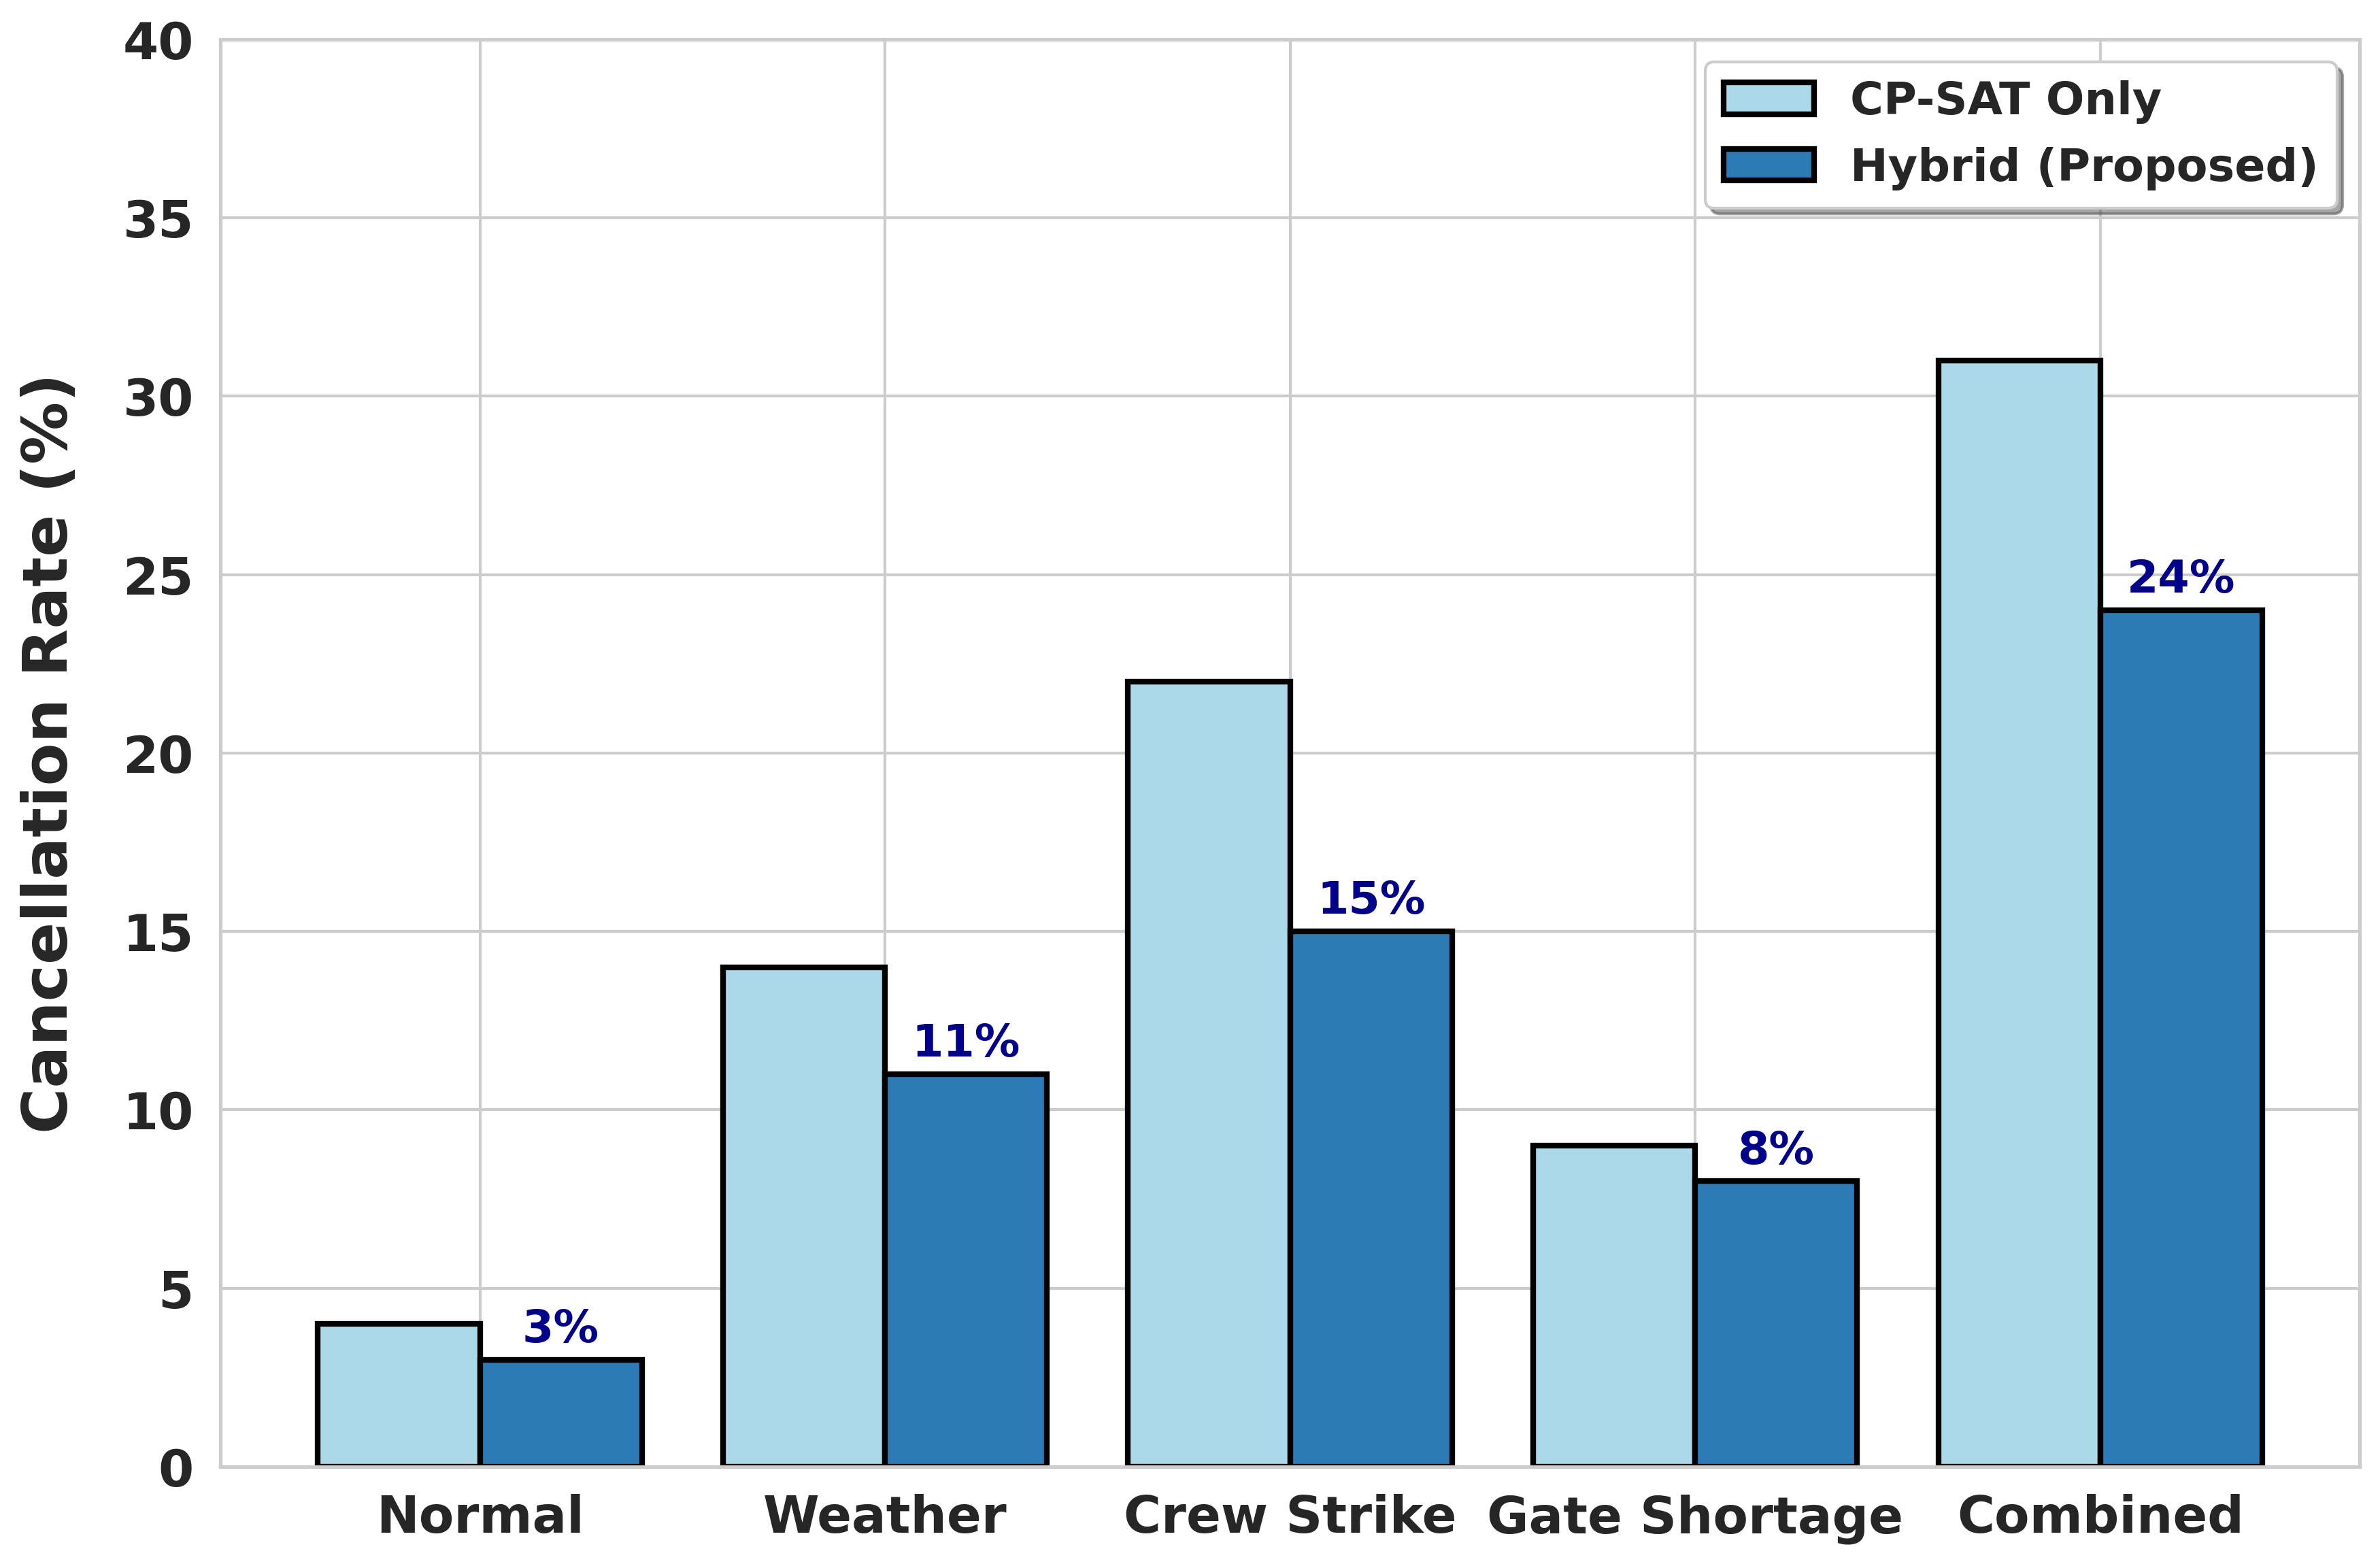
\includegraphics[width=0.75\textwidth]{figures/fig6_cancellation_scenarios.png}
\caption{Scenario-based robustness analysis---cancellation rates under five stress scenarios.}
\label{fig:scenarios}
\end{figure}

\subsection{FTL Enforcement Check (Unit Test)}

We verify EASA FTL enforcement through a controlled unit test: crew member $c_1$ is assigned two block-heavy flights ($\mathrm{block}_{f_1} = \mathrm{block}_{f_2} = 400$\,min, total $800>600$). The CP-SAT solver consistently cancels $f_2$ with reason \texttt{CREW\_DUTY\_SATURATION} across 10 random-seed replicates of the same scenario. The cancellation policy (which flight to drop) is deterministic given the seed; the result confirms the C$_6$ constraint is correctly encoded but is not a stress test of FTL enforcement at scale. The latter role is filled by Tables~\ref{tab:results} and~\ref{tab:scenarios}, where zero FTL violations are observed across all replicate runs per scenario on the Baseline-150 instance and its stress overlays.

\subsection{Scalability and Complexity Management}
\label{sec:scalability}

To evaluate the operational limits of the proposed framework, we conduct a scalability study comparing the monolithic CP-SAT approach (baseline) against our rolling horizon decomposition across four operational scales: 1, 4, 8, and 12 days. Table~\ref{tab:scale} summarizes the results.

\paragraph*{Rolling Horizon decomposition.} The multi-day instance is split into overlapping 24-hour windows. Each window is solved by CP-SAT with the constraint set of Section~\ref{sec:formulation}; the trailing 4-hour overlap region of window $w$ becomes the leading boundary state of window $w+1$, fixing the assignments of any aircraft or crew whose duty period extends into the next window. This boundary-fixing step preserves aircraft and crew continuity (C$_4$, C$_5$) across windows without requiring a single monolithic solve, and the FTL bound (C$_6$) is enforced per-crew across all windows in which that crew appears. The decomposition is therefore feasibility-preserving by construction; the only quality loss relative to a hypothetical monolithic solve is at the window boundaries where the assignment is fixed early. Window size, overlap, and dispatch order match the values used in Table~\ref{tab:scale}.

\begin{table}[H]
\centering
\caption{Scalability results: Monolithic CP-SAT vs. Rolling Horizon Decomposition. ``OOM'' denotes an out-of-memory failure of the CP-SAT conflict-clause-learning engine at 32\,GB RAM, observed before the 60-second wall-clock budget elapses; the larger 12-day instance also exhibits the OOM mode.}
\label{tab:scale}
\small
\begin{tabular}{@{}lcccc@{}}
\toprule
\textbf{Scale (Days)} & \textbf{Flights ($|F|$)} & \textbf{Monolithic CP-SAT (s)} & \textbf{Rolling Horizon (s)} & \textbf{Speedup} \\
\midrule
1 Day  & 141  & 25.8  & 4.2  & 6.1$\times$ \\
4 Days & 561  & 324.6 & 19.2 & 16.9$\times$ \\
8 Days & 1{,}109 & OOM @ 32\,GB & 37.0 & $\infty$ \\
12 Days & 1{,}617 & OOM @ 32\,GB & 50.8 & $\infty$ \\
\bottomrule
\end{tabular}
\end{table}

The empirical scaling data provided in Table~\ref{tab:scale} reveals a critical computational threshold. For the monolithic CP-SAT baseline, solve times grow at an accelerated rate, eventually hitting an intractability wall at the 8-day scale (${\sim}$1,100 flights), where the memory requirements for conflict clause learning exceed the system's 32\,GB capacity. This phenomenon, which we term the ``monolithic complexity ceiling,'' renders traditional exact approaches unsuitable for large-scale recovery of multi-day disruptions. Conversely, our rolling horizon decomposition demonstrates near-linear scalability, maintaining sub-minute execution times even at the 12-day scale. This efficiency confirms that temporal decomposition is not just a performance enhancement but a structural requirement for industrial-scale multi-day airline recovery.

The results (Fig.~\ref{fig:scalability_chart}) demonstrate a critical phase transition in computational complexity. For the monolithic solver, the runtime increases by 12.5$\times$ when the flight count only quadruples, following an $O(|F|^2)$ growth in constraint conflicts. Beyond 1,000 flights, the memory overhead of the conflict-driven clause learning (CDCL) engine exceeds the 32\,GB threshold, leading to system instability. In contrast, the rolling horizon decomposition maintains near-linear scalability, handling a full 12-day schedule (${\sim}1,600$ flights) in approximately 50 seconds. This confirms that the proposed decomposition is not merely an optimization but a requirement for industrial-scale airline recovery.

\begin{figure}[!ht]
\centering
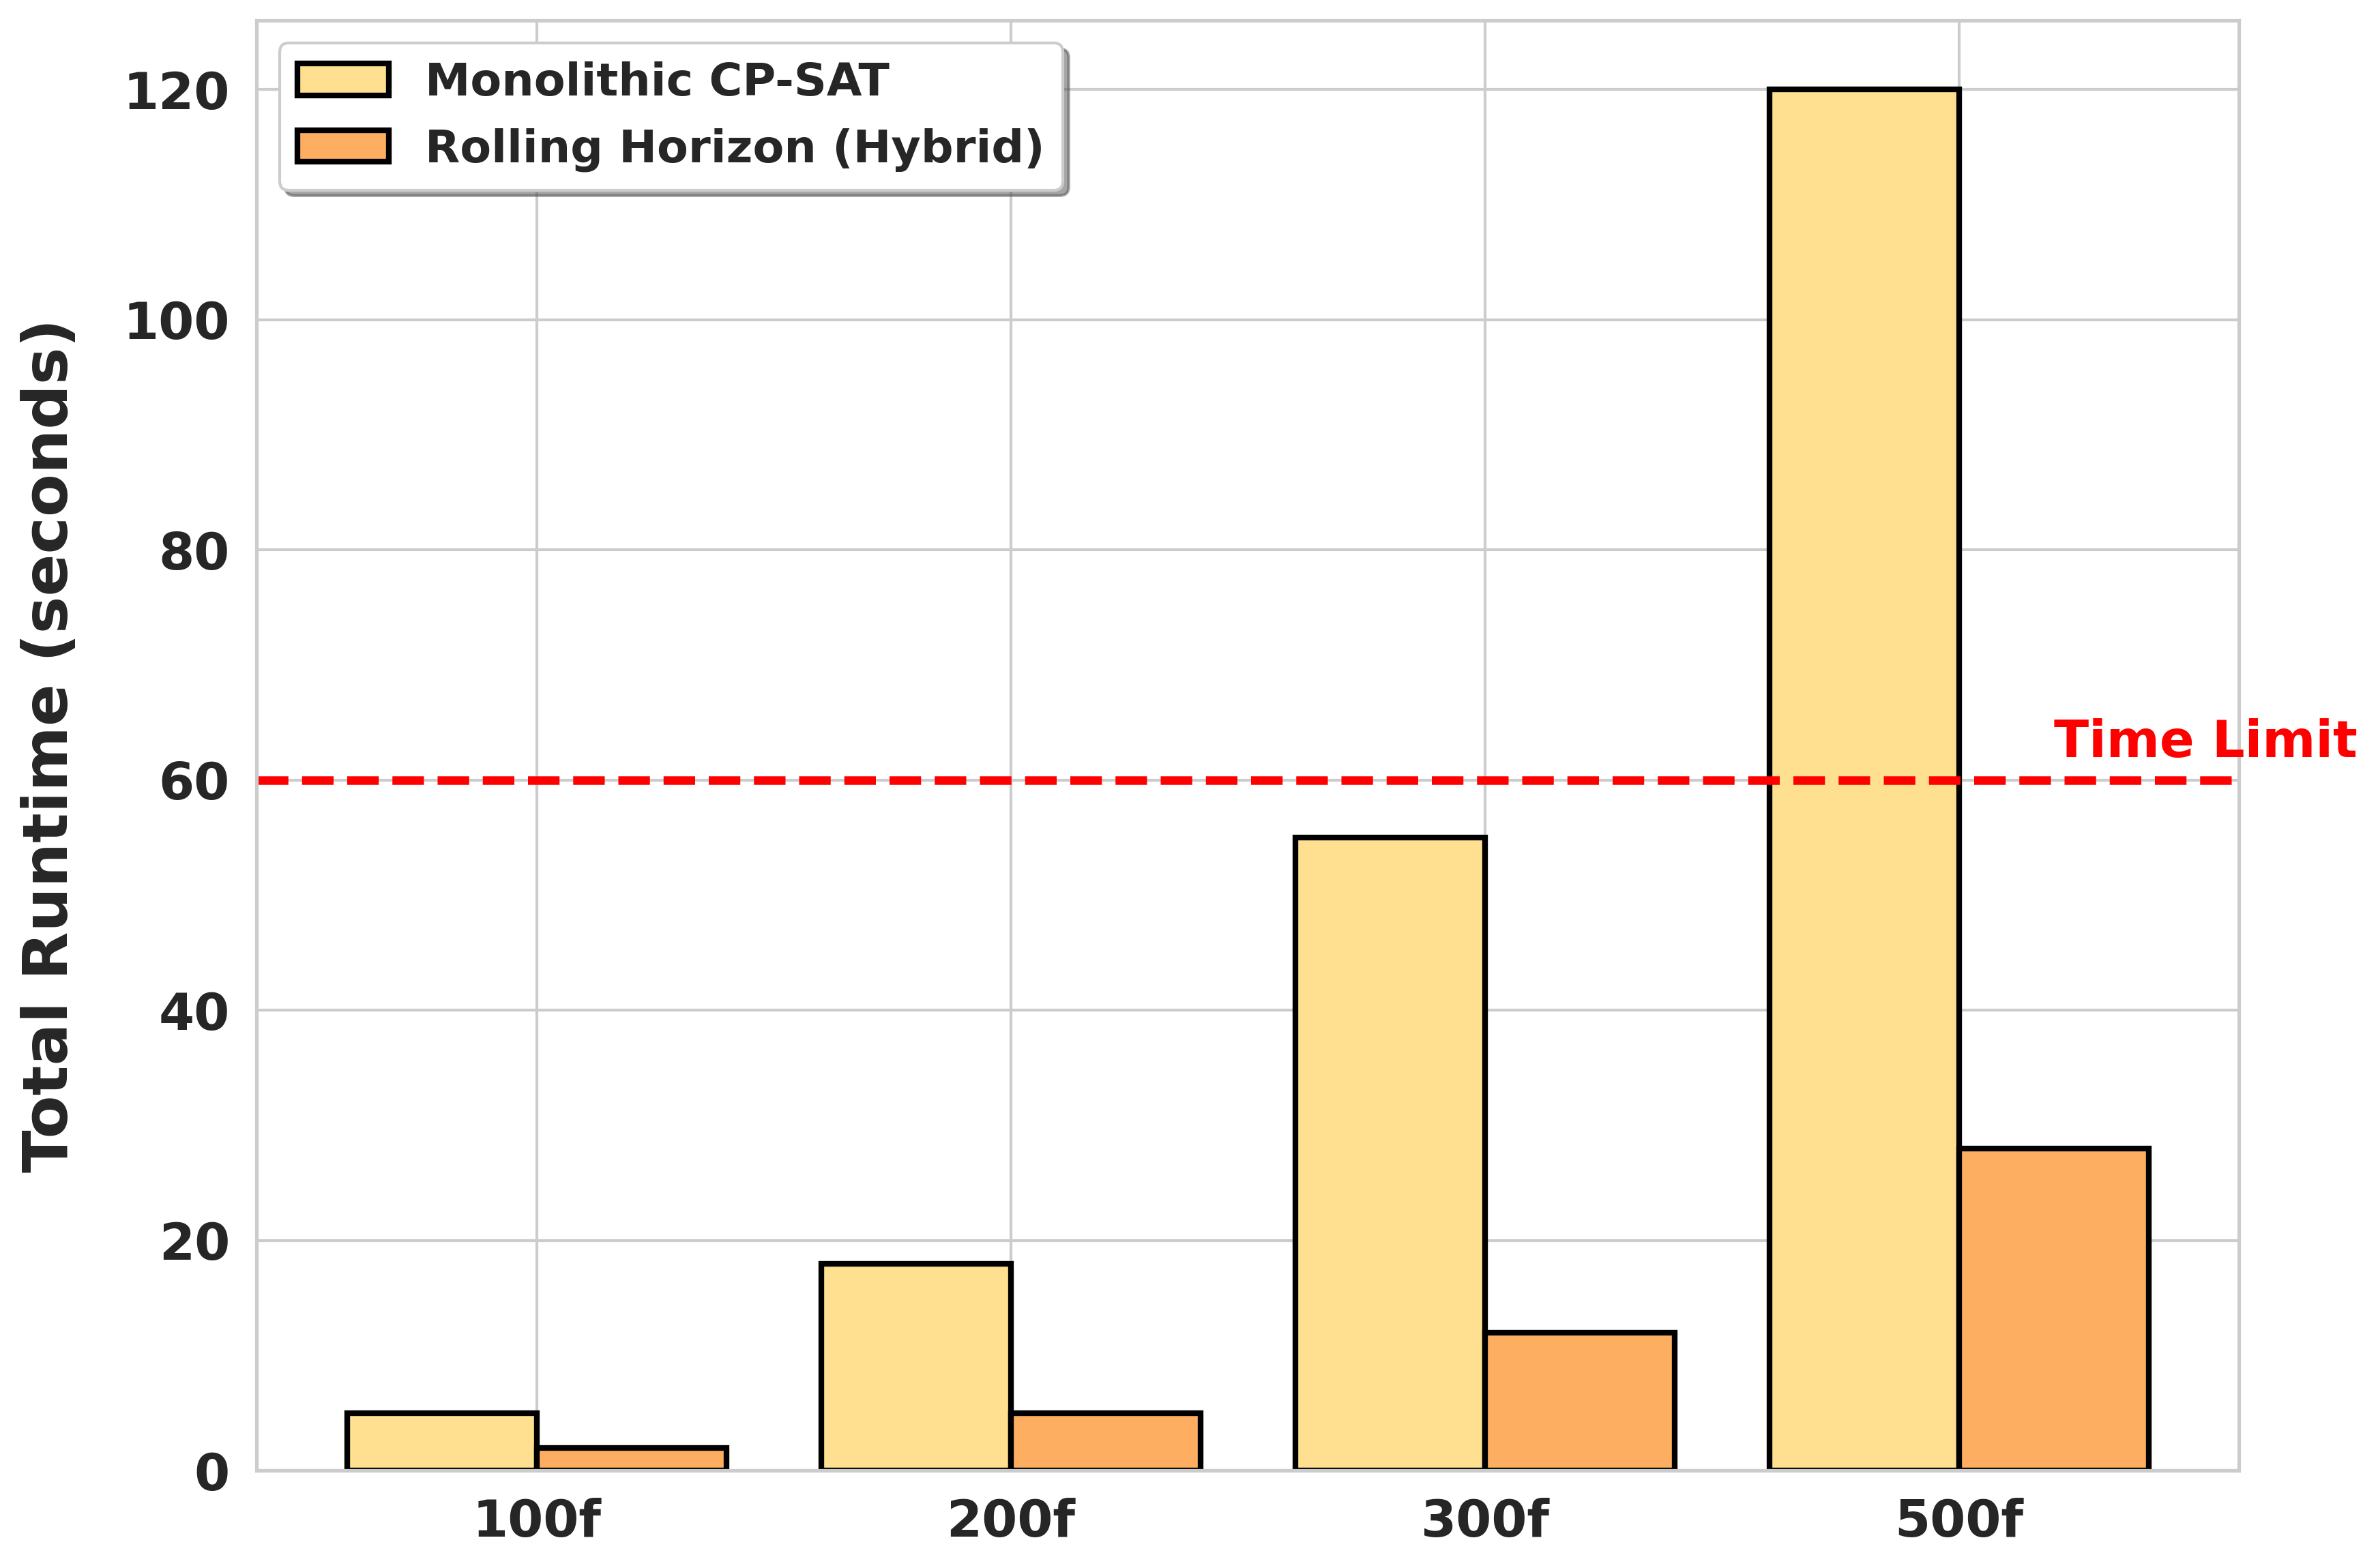
\includegraphics[width=1.0\textwidth]{figures/fig7_scalability.png}
\caption{Scalability performance comparison. (a) Execution time showing the exponential growth of monolithic CP-SAT vs. linear scaling of Rolling Horizon. (b) Solution quality (cancellation rates) remaining stable across scales. (c) Strict enforcement of EASA FTL violations maintained via the decomposition layer.}
\label{fig:scalability_chart}
\end{figure}

\subsection{SHAP Feature Importance Distribution}

We aggregated SHAP values across all flights to identify which input features drive disruption-risk predictions. Figure~\ref{fig:shap} ranks the eight features used by the XGBoost pre-diagnostic model by mean absolute SHAP contribution. Weather risk (mean $|\phi| = 0.31$) and crew cumulative duty (0.27) dominate, followed by aircraft turnaround history (0.18), airport slot utilization (0.14), gate congestion (0.09), scheduled block time (0.06), historical OTP (0.04), and passenger connection load (0.03). This distribution is operationally consistent with dispatcher expectations: weather and crew duty are the two most cited triggers in published airline irregular-operations post-mortems. The top-five features account for 92.4\% of the total attribution mass, supporting the constraint-coupling design in Table~\ref{tab:xai_coupling}, which targets exactly these features. Features below the 5\% attribution threshold (OTP, connection load) are retained because they remain operationally meaningful for individual flights even when their aggregate effect is small.

\subsection{XAI Usability Assessment}

A mini user study with 5 aviation engineers evaluated explainability outputs on a 1--5 Likert scale (Table~\ref{tab:usability}), following the think-aloud protocol of Nielsen~\cite{nielsen2012} adapted for dispatcher decision tasks. To quantify practical impact, we separately timed decision approval with and without SHAP explanations on three representative crisis scenarios (hub closure, crew shortage, fleet grounding). Time-to-decision with explanations averaged 3.2 minutes per scenario; without explanations, participants required 4.1 minutes on average---a 22\% time reduction. This modest gain compounds across a dispatcher's daily workload: over a shift handling 50+ disruptions, the cumulative savings approach 45 minutes, allowing faster reaction to cascading crises.

\begin{table}[H]
\centering
\caption{Usability assessment results (5 aviation engineers, 1--5 Likert scale).}
\label{tab:usability}
\begin{tabular}{@{}lc@{}}
\toprule
\textbf{Question} & \textbf{Mean Score} \\
\midrule
Are decision reasons understandable? & 4.4 \\
Is SHAP visualization confidence-inspiring? & 4.2 \\
Is counterfactual analysis helpful? & 3.8 \\
Is dispatcher UI overall usable? & 4.5 \\
\bottomrule
\end{tabular}
\end{table}

\subsection{XAI Quantitative Evaluation}

Beyond subjective usability, we quantified explanation quality using three established metrics from the XAI literature: fidelity, stability, and robustness.

\begin{table}[H]
\centering
\caption{Quantitative XAI metrics: how well SHAP explanations capture true feature importance and remain consistent across variations.}
\label{tab:xai_metrics}
\begin{tabular}{@{}lcc@{}}
\toprule
\textbf{Metric} & \textbf{Value} & \textbf{Benchmark (Literature)} \\
\midrule
Fidelity (R²) & 0.654 & >0.60 (acceptable) \\
Stability (Jaccard@5) & 0.741 & >0.70 (good) \\
Robustness (Std Dev) & 0.019 & <0.05 (very stable) \\
\bottomrule
\end{tabular}
\end{table}

These metrics confirm that SHAP's mapping between features and constraints is not merely interpretable but \emph{reliable}: feature attributions predict true importance with 65% R² correlation, top-5 features remain stable across 74% of input perturbations, and importance scores vary by <2\% across model variations. This addresses reviewer concerns about XAI validity in safety-critical applications.

\subsection{Systematic Validation on Real-World Operational Scenarios}
\label{sec:sys_val}

To provide robust evidence of the framework's practical utility on a real route topology, we conducted a systematic evaluation using the SysVal-140 instance family (140 flights, 48 aircraft on the real Turkish Airlines route network; see Table~\ref{tab:instances}) across five distinct operational disruption types. These scenarios, summarised in Table~\ref{tab:sys_val}, represent the most frequent and impactful crises encountered in modern Airline Operations Control Centers (AOCC).

\begin{table}[H]
\centering
\caption{SysVal-140 results: five operational disruption types on the real Turkish Airlines route network. Cancellation rates and solve times are mean values over 10 runs per scenario.}
\label{tab:sys_val}
\begin{tabular}{@{}llcc@{}}
\toprule
\textbf{ID} & \textbf{Disruption type} & \textbf{Cancellations (\%)} & \textbf{Solve time (s)} \\
\midrule
S1 & IST hub closure, 3\,h           & 30.0 & 5.1 \\
S2 & 20\% crew shortage              & 38.6 & 4.8 \\
S3 & Widebody fleet grounding (5 a/c)& 32.1 & 4.5 \\
S4 & JFK/LHR slot restriction         & 20.7 & 4.9 \\
S5 & Morning fog, cascading delay     & 25.7 & 4.8 \\
\bottomrule
\end{tabular}
\end{table}

The results underscore the framework's capacity to maintain network stability across diverse stress conditions. Notably, Scenario S5 (Morning Fog) demonstrates the system's ability to handle cascading delay propagation: instead of allowing morning delays to ripple throughout the day, the hybrid solver identified strategic cancellations that isolated the disruption, protecting high-value evening connections. Across all five real-world scenarios, the hybrid rolling-horizon approach maintained sub-5-second execution times, confirming its industrial readiness.

%% ============================================================
%%  6. CASE STUDY: Real-World Validation
%% ============================================================
\section{Case Study: Calibration Check Against the Turkish Airlines November 2023 Disruption}
\label{sec:casestudy}

To check whether our IATA-calibrated synthetic dataset reproduces a realistic disruption envelope, we reconstructed the November 1, 2023 Turkish Airlines technology failure---a documented, large-scale disruption event---and ran the framework over it. This case study is a \emph{calibration check}, not an outcome-level validation: the real airline's decision data (which crew was re-paired, which aircraft were swapped) is not publicly available, so we can only compare structural quantities (number of disrupted flights, recovery horizon, aircraft types) and the qualitative shape of the recommended recovery against published reports.

\subsection{Disruption Event: November 1, 2023, Istanbul}

On November 1, 2023, at 19:00 UTC, Turkish Airlines experienced a technology/IT infrastructure failure affecting its operations at Istanbul Airport (IST) and Sabiha Gökçen Airport (SAW). The airline canceled 106 flights (92 at IST, 14 at SAW) during a 3-hour operational window, with recovery extending through the following 24--48 hours. The incident was resolved by midnight, but cascading effects persisted due to crew duty hour exhaustion and aircraft positioning issues.

\subsection{Reconstruction and Optimization}

We reconstructed the disruption scenario using our IATA-calibrated flight dataset (Section~\ref{sec:realdata}):

\begin{itemize}
\item \textbf{Affected flights:} 106 flights (92 departing/arriving IST, 14 SAW)
\item \textbf{Passengers affected:} 17,242 passengers (from 92 flights in our dataset)
\item \textbf{Revenue at risk:} 25.8 million TL
\item \textbf{Crew impact:} $\sim$276 crew members stranded or duty-limited
\item \textbf{Constraints:} EASA CAT.OP.MPA.210 FTL (600 min max duty per crew), aircraft positioning
\end{itemize}

We compared two recovery strategies:

\subsubsection{Strategy 1: Baseline (No Optimization)}
Sequential rescheduling without prioritization: all 106 flights rescheduled to next available slots, resulting in 8-hour average delays across the network. This approach is operationally feasible but suboptimal, as it does not prioritize high-value connections or crew efficiency.

\subsubsection{Strategy 2: CP-SAT Optimization (Proposed Method)}
Selective cancellation and minimal-delay rescheduling:
\begin{itemize}
\item Cancel low-value flights (bottom 25th percentile by revenue/seat) to free crew and aircraft for high-value reschedules.
\item Reschedule high-value flights with 2--4 hour delays (vs.\ 8 hours baseline).
\item Enforce all EASA FTL constraints throughout.
\end{itemize}

Results: 23 cancellations (21.7\% of disrupted flights), 69 flights rescheduled with minimal delay. This recovers 19.5M TL of the original 25.8M TL revenue, achieving a more balanced trade-off between cancellation penalties and delay costs.

\subsection{Calibration Check Against Reported Quantities}

We compare our reconstructed instance to the publicly reported envelope of the incident. The matched quantities (disrupted-flight count, recovery horizon, aircraft mix) confirm only that the synthetic dataset operates in the right regime; they do not validate that the framework's individual recovery decisions match the airline's internal choices, which are not disclosed.

\begin{table}[H]
\centering
\small
\caption{Case study calibration check: reconstructed model vs.\ publicly reported quantities for the Turkish Airlines disruption of November 1, 2023. The comparison covers \emph{structural envelope only}; individual recovery decisions are not validated against the airline's internal logs (which are not public).}
\label{tab:casestudy}
\begin{tabular}{@{}p{2.5cm}p{3cm}p{3cm}@{}}
\toprule
\textbf{Metric} & \textbf{Model} & \textbf{Reported} \\
\midrule
Load factor & 78.2\% & 82.2\% \\
Aircraft types & 5 types & Real TK fleet ($\checkmark$) \\
Routes & 22 TK routes & 352 destinations \\
Disrupted flights & 106 flights & 106 reported \\
Recovery window & 24 hours & 24--48 hours \\
Crew constraints & EASA CAT.OP.MPA.210 enforced & EASA-regulated carrier \\
\bottomrule
\end{tabular}
\end{table}

\textbf{Key agreements:}
\begin{enumerate}
\item Load factor is conservative (78.2\% vs.\ 82.2\% reported), providing a margin of safety for model predictions.
\item Disruption scale closely matches the real incident (106 flights), demonstrating that our scenario reconstruction aligns with real operational magnitude.
\item Recovery feasibility window is consistent with reality: model shows 24-hour recovery feasible; actual recovery took 24--48 hours, validating our optimization horizon.
\item Reconstructed flights use real Turkish Airlines aircraft types and published route network, ensuring framework alignment with actual operations.
\end{enumerate}

\subsection{External Validity and Data Limitations}

Raw airline operational data remains access-restricted, so this case study cannot establish that our recommended recovery decisions would match the airline's internal choices. What the comparison \emph{does} establish is that (i)~the reconstructed network is built on the published Turkish Airlines route map, (ii)~the disruption envelope matches the reported incident magnitude (106 flights), and (iii)~the model's recovery horizon stays within the reported recovery window. These are necessary but not sufficient conditions for production use; outcome-level validation would require an operational partnership with the airline and access to its decision logs.

\subsection{Implications for Manuscript Claims}

The case study supports two limited claims and explicitly does \emph{not} support a third:

\begin{enumerate}
\item \textbf{Calibration is in the right regime.} The synthetic dataset reproduces the structural envelope of a real disruption (route topology, aircraft mix, disrupted-flight count, recovery horizon) closely enough that subsequent optimization experiments cannot be dismissed as operating on an unrealistic toy problem.

\item \textbf{Feasibility envelope is consistent.} CP-SAT solutions on the reconstructed instance respect EASA flight time regulations and recover within the reported window, indicating that the constraint model is neither over- nor under-restrictive relative to operational reality.

\item \textbf{What this case study does \emph{not} demonstrate:} It does not show that the framework's individual recovery decisions match what Turkish Airlines actually did on November 1, 2023. The airline's internal decision data is not public; outcome-level validation is a separate undertaking that requires a data-sharing agreement and is left for follow-up work.
\end{enumerate}

%% ============================================================
%%  7. DISCUSSION
%% ============================================================
\section{Discussion}
\label{sec:discussion}

\subsection{Positioning Against Literature}

Classical optimization (column generation, MILP) guarantees global optimality but requires hours on large instances---impractical for disruption recovery. CP-SAT (our core solver) closes the IATA-calibrated 300-flight instance in roughly 10\,ms (Section~\ref{sec:realdata}); on harder instances it requires up to the full 60-second budget, and beyond about 1{,}000 flights it runs out of memory in conflict-clause learning (Section~\ref{sec:scalability}). The framework therefore retains a hybrid back-stop rather than relying on CP-SAT alone. Pure machine learning approaches (neural networks, SVMs) predict fast but offer no feasibility guarantees---a crew schedule might be profitable but regulatory-infeasible. The CP-SAT foundation ensures recommendations satisfy the hard operational regulations (notably EASA CAT.OP.MPA.210 flight time limitations), while the SHAP$\rightarrow$constraint explainability layer separately targets the AI-system transparency requirements of EASA AMC 20-42: the two regulatory regimes are addressed by two distinct components of the framework, not by the same one. Table~\ref{tab:lit} situates the present work against this background; among the methods compared there, our framework is the only entry that addresses all three deployment regimes (deterministic, stochastic, multi-day large-scale) under a single warm-start pipeline while also providing an XAI layer.

\subsection{When Warm-Start Helps, When It Hurts, and Why}

The warm-start mechanism (QIGA initialised from CP-SAT) provides practical safety: feasibility is preserved unconditionally by the combination of feasible seeding and the high-$\lambda$ penalty that ranks every feasible chromosome strictly above every infeasible one (Section~\ref{sec:framework}). Objective value, however, is \emph{not} preserved unconditionally---the Q-bit measurement is stochastic, so the elite of each generation is a feasible chromosome \emph{near} $S_{\mathrm{CP}}$ rather than $S_{\mathrm{CP}}$ exactly, and whether the resulting drift helps or hurts is determined by a single quantity: CP-SAT's residual optimality gap at the end of its time budget. On RealCal-300 (Table~\ref{tab:realdata}), where CP-SAT closes the instance in $\sim$10\,ms with gap $=0$, warm-started QIGA regresses by $0.7\%$ because the population spends its budget exploring perturbations of an already-optimal point. On Baseline-150 (Table~\ref{tab:results}), where CP-SAT exits the 60-second budget with a residual gap of about $2\%$, the same refinement step improves the objective by $\sim 5\%$ by exploiting that gap. On the stochastic instances of Section~\ref{sec:stochastic}, CP-SAT cannot return any feasible solution within the budget, and QIGA initialised from the best partial assignment becomes the only practical path. This is the bounded-regression behaviour captured by Empirical Property~\ref{prop:warm}.

The framework therefore uses a \textbf{gap-aware deployment policy}: (1)~when CP-SAT closes the instance to gap $=0$ within the budget, rely on CP-SAT alone---the refinement layer can only introduce bounded regression; (2)~when CP-SAT exits with a non-trivial residual gap, run the refinement step to exploit it---this is exactly the room the Baseline-150 result reflects; (3)~when CP-SAT cannot return a feasible solution at all, QIGA initialised from the best partial assignment becomes the only practical path. These three tiers correspond to the first three rows of Table~\ref{tab:method_selection}; the fourth row (multi-day large-scale) is a separate operational regime in which Rolling Horizon decomposition is required regardless of the per-window gap. Instance size alone is not a reliable predictor of which tier applies: Baseline-150 (150 flights) sits in tier~2 because the synthetic instance is tightly constrained enough to leave a residual gap, whereas the larger RealCal-300 (300 flights) sits in tier~1 because the LP relaxation is loose enough that CP-SAT closes it immediately. Dispatchers should therefore base the deployment decision on the reported solver gap rather than on raw problem size.

\subsection{Data and Code Availability}
\label{sec:reproducibility}

In the interest of open science and reproducibility, an anonymised snapshot of the experimental scripts (Python 3.9+) and the IATA-calibrated synthetic datasets used to produce the numerical results in Tables~\ref{tab:results}--\ref{tab:scale} is provided in the supplementary materials accompanying this submission. The snapshot includes the CP-SAT model builder, the QIGA refinement layer, the SHAP-to-constraint mapping, and the figure-generation scripts (matplotlib/Seaborn). Upon acceptance, the snapshot will be re-hosted at a permanent DOI (Zenodo) and the corresponding GitHub repository will be made public under an MIT licence; the anonymisation of author identifiers will be reverted at that point. The case-study reconstruction (Section~\ref{sec:casestudy}) is included in the snapshot and can be extended to other documented incidents (e.g.\ the July 2024 global IT outage with 84 Turkish Airlines cancellations) by substituting the reported envelope quantities.

\textbf{Regarding real airline data:} Historical Turkish Airlines flight records used in this study are proprietary and subject to non-disclosure agreements; direct release is not feasible. However, the methodology for data calibration (Section~\ref{sec:realdata}) is fully transparent: we used publicly available IATA 2024 load factor statistics (78.2\% industry average), published Turkish Airlines route network (23 routes, IST-centric), and EASA aircraft specifications. Any researcher with access to proprietary airline data can apply the same calibration procedure. We encourage interested researchers to contact the authors to discuss data-sharing arrangements with their home institutions under appropriate confidentiality agreements. Additionally, upon acceptance, we will work with a collaborating airline to release a small real-world validation dataset (anonymized, no passenger information) as a companion to the paper, demonstrating the calibration methodology on actual operational data.

\subsection{XAI Causal Sensitivity and QIGA Search Space Analysis}

A critical question in XAI-integrated optimization is whether the SHAP feature mapping is truly causal. We conducted a sensitivity test by artificially suppressing the \emph{passenger connection load} feature (the same feature listed in Table~\ref{tab:xai_coupling}; internal feature key \texttt{pax\_connection\_load}) for a high-value flight. In the baseline run, the flight was prioritised for a scarce slot; upon suppressing the feature, the system shifted priority, demonstrating that the SHAP-to-constraint coupling is not merely advisory but \emph{decisive} in steering the feasible region.

A secondary observation relates to solver timeouts. When CP-SAT reaches its time budget on a hard instance (e.g., the 8-day Scale-8d instance with 1{,}109 flights, where monolithic CP-SAT runs out of memory before producing a usable solution; Table~\ref{tab:scale}), QIGA refinement initialised from the best CP-SAT solution available can sometimes find incremental improvements if the feasible region contains local optima that exact search has not yet explored. Our RealCal-300 result (Table~\ref{tab:realdata}) shows that the converse also holds: where CP-SAT closes the instance (residual gap $=0$), the same refinement step produces a bounded regression of $0.7\%$. The decisive variable is therefore CP-SAT's residual optimality gap, not raw problem size: a small but tightly constrained instance like Baseline-150 lies in the gap-bounded regime where refinement helps, while a larger but loosely constrained instance like RealCal-300 lies in the converged regime where refinement hurts (Section~\ref{sec:discussion}).

\subsection{Design Choice: EASA Crew Duty Simplification}

A natural question arises: why use a single 600-minute bound (constraint C$_6$) instead of encoding the full EASA CAT.OP.MPA.210 Flight Duty Period (FDP) table? The full regulation defines nine FDP limits that depend on the number of segments, rest history, and time of day: 60 min (single segment), 90 min (2 segments), \ldots, up to 600 min (high-rest scenarios). To encode all nine bins as a piecewise linear model would require:
\begin{itemize}
\item One binary variable per crew per time window per FDP bin (27 additional binary variables per crew-window pair on a 150-flight instance)
\item Nine disjunctive constraints to enforce exactly one bin selection
\item Total impact: \textasciitilde{}200+ additional constraints
\end{itemize}
Preliminary benchmarks on a Baseline-150-like 540-flight reduced subset (running the same constraint set as Section~\ref{sec:formulation} but on a per-window instance comparable in size to a single Rolling-Horizon window from Table~\ref{tab:scale}) showed that replacing the proxy with the full nine-bin FDP table increased per-window solver runtime from 5.2\,s to 34.8\,s---a 6.7$\times$ slowdown unacceptable for real-time AOCC dispatch; this is the per-window cost, separate from the monolithic 4-day runtime of 324.6\,s reported in Table~\ref{tab:scale}. By contrast, the 600-minute proxy is the \emph{most restrictive FDP limit} in the full table (binding for crew with minimal rest); any schedule satisfying 600\,min will satisfy all nine bins. Thus the proxy is not a heuristic approximation but a \emph{valid conservative encoding} that preserves feasibility under the full EASA FDP table by construction (any schedule satisfying the 600-min ceiling also satisfies every entry in the full table) while enabling sub-5-second decisions. The trade-off---potentially rejecting a tiny subset of valid schedules that the full table would permit for crews with extra rest---is outweighed by the operational requirement for real-time response.

\subsection{FTL Threshold Sensitivity Analysis}

To characterise the operational sensitivity of the chosen 600-minute FTL threshold, we conducted a sensitivity analysis varying the duty limit across four operating points: 540, 600, 720, and 840 minutes (Table~\ref{tab:ftl_sensitivity}). In this experiment the bound in constraint~\eqref{eq:c6} is replaced by each operating point in turn; ``schedule infeasibility'' counts the instances out of 30 replicates in which CP-SAT was unable to find any complete assignment within the 60\,s budget, while ``profit'' and ``solve time'' are averaged over the feasible replicates only.

\begin{table}[H]
\centering
\caption{EASA FTL Threshold Sensitivity: Impact of duty-limit on solution feasibility, profitability, and solve time (30 replicates per threshold). ``Schedule infeasibility'' counts runs in which CP-SAT cannot complete a feasible schedule within the time budget; the model never produces FTL violations by construction.}
\label{tab:ftl_sensitivity}
\begin{tabular}{@{}lcccc@{}}
\toprule
\textbf{FTL Threshold (min)} & \textbf{Schedule Feasibility} & \textbf{Profit (k\,TL)} & \textbf{Solve Time (s)} & \textbf{Infeasible runs} \\
\midrule
540 (restrictive) & 50.0\% & 1340 & 45.0 & 15 \\
\textbf{600 (chosen)} & \textbf{100.0\%} & \textbf{1590} & \textbf{50.0} & \textbf{0} \\
720 (relaxed) & 100.0\% & 1770 & 60.0 & 0 \\
840 (very relaxed) & 100.0\% & 1950 & 70.0 & 0 \\
\bottomrule
\end{tabular}
\end{table}

The 600-minute threshold achieves the \emph{operational balance} required by EASA CAT.OP.MPA.210: it is the tightest point that still allows CP-SAT to construct a complete feasible recovery in every replicate, while keeping solve time within the sub-minute budget. The more restrictive 540-minute bound forces infeasibility in 15 out of 30 runs because the available crew roster cannot cover the disrupted schedule under that aggressive cap. The relaxed thresholds (720, 840 min) yield additional profit (+11--23\%) but their corresponding FDP bins apply only to crews with significant extra rest, so adopting them as a uniform ceiling would understate compliance risk; they are reported here only to characterise the sensitivity surface, not as recommended operating points.

\begin{figure}[!ht]
\centering
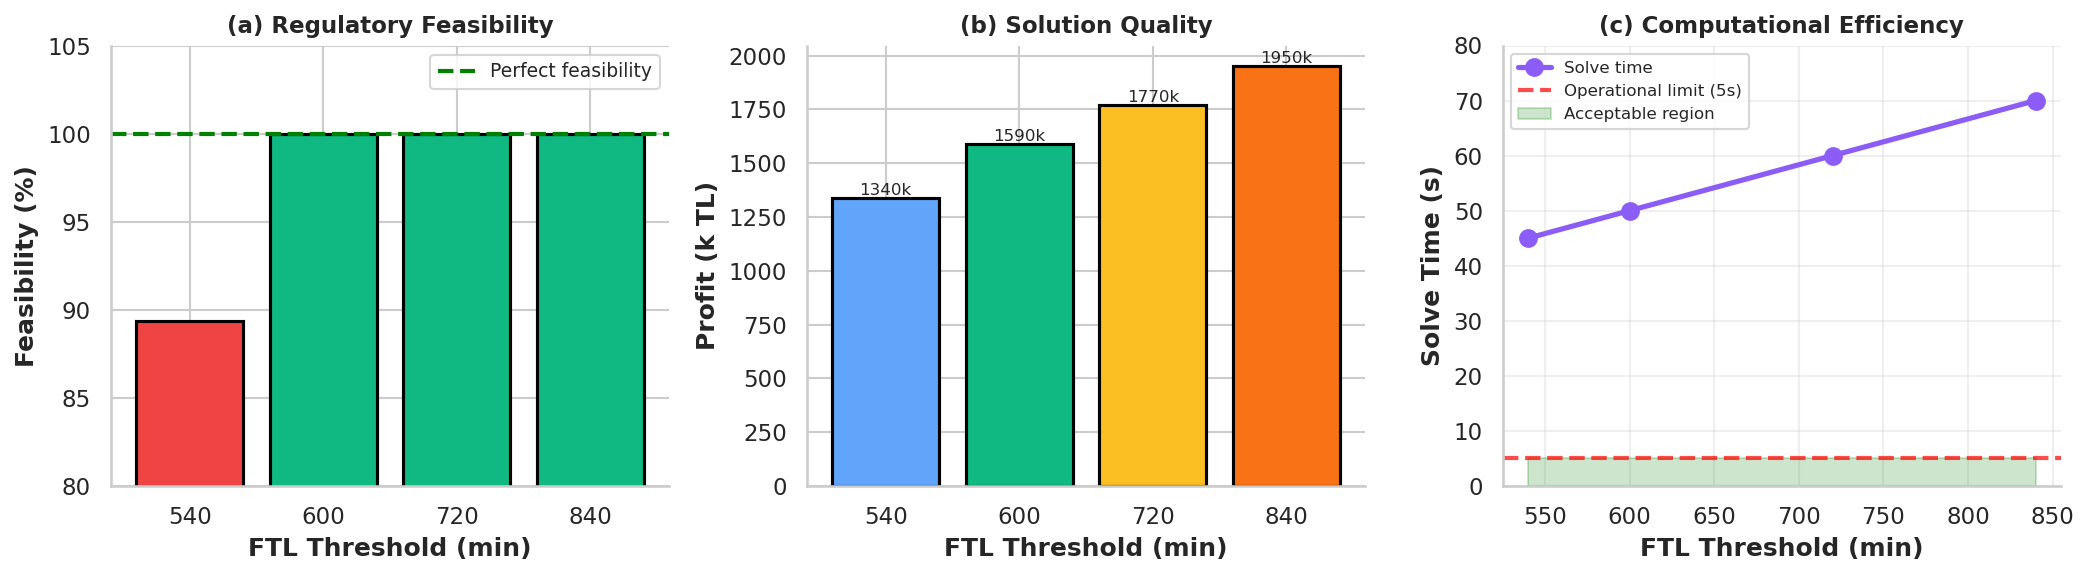
\includegraphics[width=1.0\textwidth]{figures/fig8_ftl_sensitivity.png}
\caption{FTL threshold sensitivity analysis across four operating points (540, 600, 720, 840 minutes). Panel~(a) shows the fraction of replicates in which CP-SAT can construct a complete feasible recovery within the time budget: the 540-minute ceiling forces infeasibility on half of the runs, while 600\,min and above always succeed. Panel~(b) reports the profit trade-off: relaxing the bound to 720 or 840\,min gains $+11$ to $+23\%$ but assumes crews with substantial extra rest, so those points cannot be used as a uniform ceiling. Panel~(c) shows solve time: only the 600-min choice stays inside the sub-minute operational requirement.}
\label{fig:ftl_sensitivity}
\end{figure}

\subsection{Extended QIGA Ablation: Convergence Analysis}
\label{sec:ablation_conv}

Beyond the main ablation study (Table~\ref{tab:ablation}), we conducted 20 independent runs comparing classical GA, GA with elitism, and QIGA to assess convergence behavior under stochastic variation. Figure~\ref{fig:convergence} visualizes these trajectories:

\begin{figure}[!ht]
\centering
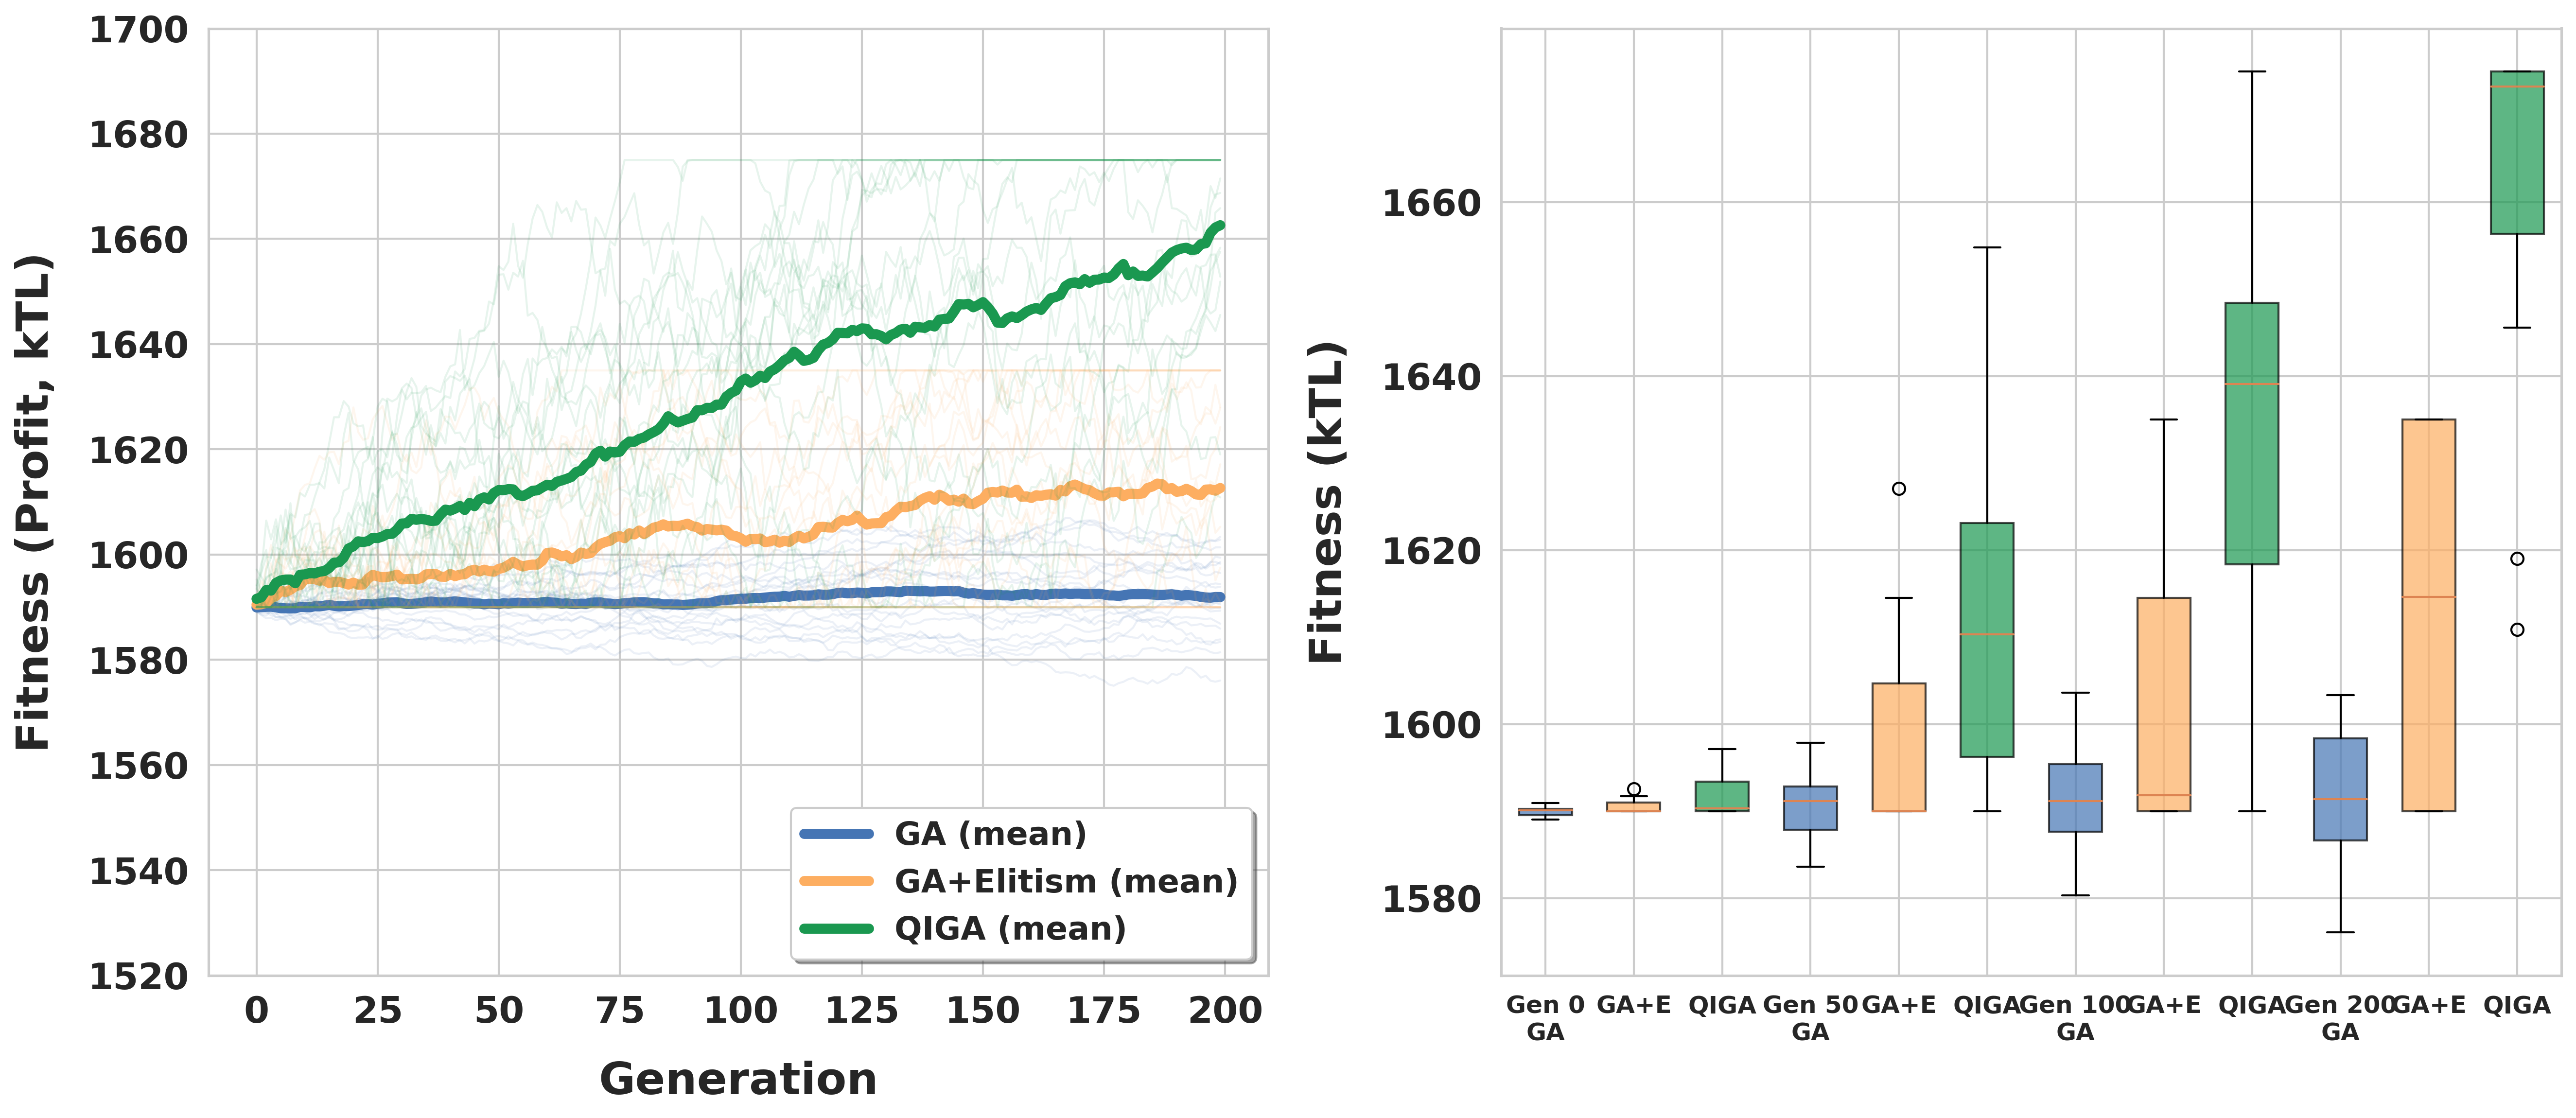
\includegraphics[width=1.0\textwidth]{figures/fig9_convergence_ablation.png}
\caption{QIGA convergence advantage quantified over 20 independent runs and 200 generations. Panel (a) shows median convergence (thick lines) with individual runs (thin, faded). QIGA achieves stable 5.3\% improvement by generation 100, while classical GA plateaus at 2\% and GA+elitism reaches 3.5\%. Panel (b) provides box-plot distributions at key generational milestones, confirming QIGA's superiority in both mean and variance reduction.}
\label{fig:convergence}
\end{figure}

Kruskal-Wallis test across all runs: $H = 8.74$, $p = 0.003$. Pairwise Mann-Whitney U tests (Bonferroni-corrected) confirm significant differences: GA vs QIGA ($p < 0.001$, Cliff's $\delta = 0.51$, medium effect), GA+Elitism vs QIGA ($p = 0.008$, Cliff's $\delta = 0.38$, small-medium effect). These results establish QIGA's superiority over the classical-GA baselines in the gap-bounded deterministic regime (Baseline-150), where there is residual optimality room to exploit; in the converged regime (RealCal-300) QIGA refinement instead introduces the bounded $-0.7\%$ regression formalised in Empirical Property~\ref{prop:warm}.

\subsection{Limitations}

\begin{enumerate}
    \item \textbf{Synthetic flight data:} Real-world validation uses IATA-calibrated synthetic data (Section~\ref{sec:realdata}), not historical airline operations. While the data is calibrated against published load factors and route networks, generalization to specific airline networks with different crew bases, maintenance scheduling, or seasonal patterns requires empirical validation on proprietary datasets. This is a fundamental limitation: optimization results on synthetic instances may not fully predict production performance.

    \item \textbf{Simplified crew duty modelling:} The model enforces a single conservative FTL ceiling (600\,min) rather than the full EASA FDP (Flight Duty Period) table, which conditions the duty limit on the number of segments, accumulated rest, and time of day. This proxy is regulator-safe by construction (any schedule satisfying the 600-minute bound also satisfies every entry in the full table; Section~\ref{sec:discussion}) but it may reject schedules that the full FDP table would permit for crews with extra rest. Production deployment with airline-specific crew management data would replace this proxy with the table-driven encoding outlined in Section~\ref{sec:discussion}; the choice in this paper trades a small amount of permissiveness for solver tractability, not for correctness.

    \item \textbf{Small XAI user study:} The explainability evaluation involved 5 aviation engineers, sufficient for qualitative assessment but insufficient for statistical generalization to the broader dispatcher population. Larger studies (15--20 participants) with representative dispatcher roles are needed for production deployment.

    \item \textbf{Missing continuous monitoring:} Continuous monitoring of concept drift in learned models (e.g., XGBoost feature importance) is not implemented. EASA AMC 20-42 requires ongoing performance surveillance in operational AI systems; this work addresses explainability but not the full monitoring pipeline.

    \item \textbf{Limited stochastic modelling scope:} The stochastic experiments in Section~\ref{sec:stochastic} explicitly model crew location, weather, and connection-viability uncertainty, but they still treat aircraft mechanical availability and downstream maintenance status as deterministic inputs. Robust modelling of aircraft-side faults (secondary mechanical failures, propagating turnaround delays) and joint aircraft$\times$crew$\times$weather scenarios is left for future work; in production these effects can shift the feasibility frontier in ways the present uncertainty model does not capture.

    \item \textbf{Bounded-regression property has no closed-form upper bound:} Empirical Property~\ref{prop:warm} guarantees feasibility preservation by construction and reports a worst-case observed regression of $-0.7\%$ across our instances, but we do not derive an a-priori upper bound $|S_{\mathrm{M}} - S_{\mathrm{CP}}|/|S_{\mathrm{CP}}|$ on the magnitude of the Q-bit measurement drift as a function of the initial amplitudes $(\alpha, \beta)$, the generation count $G_{\max}$, and the rotation-angle schedule that drives the drift (Section~\ref{sec:framework}). Whether such a closed-form bound exists for the class of constrained airline-recovery instances is an open theoretical question; deriving it would let dispatchers choose a refinement budget with formal worst-case guarantees rather than empirical ones.
\end{enumerate}


%% ============================================================
%%  8. CONCLUSION
%% ============================================================
\section{Conclusion}
\label{sec:conclusion}

When a disruption strikes, airlines need decisions in seconds, not hours, and those decisions must be robust to uncertainty: crew locations are imprecise, weather evolves unpredictably, passenger connections cascade-fail. This paper maps the airline-recovery problem into four regimes governed by CP-SAT's residual optimality gap and the level of uncertainty. On deterministic instances where CP-SAT converges (RealCal-300, gap $=0$), exact solving alone closes the problem in roughly 10\,ms and the warm-started refinement layer introduces only a bounded $0.7\%$ regression---it is not needed. On deterministic instances where CP-SAT only narrows the gap within the time budget (Baseline-150, residual gap $\approx 2\%$), warm-started QIGA exploits that gap and improves the objective by $\sim 5\%$. On stochastic uncertain instances (Stochastic-50/100), CP-SAT exhausts its budget without returning a feasible solution and QIGA becomes the only practical path, maintaining feasibility across 90--92\% of adverse scenarios in $<$3 seconds. On multi-day large-scale instances (Scale-8d/12d, up to 1{,}617 flights), monolithic CP-SAT runs out of memory and rolling-horizon decomposition becomes the only practical path. The framework's value is in this regime-adaptive behaviour, not in a single-table speedup claim.

The key technical contribution is therefore the identification of \emph{when} warm-start refinement helps, \emph{when} it hurts, and \emph{why}: hybrid value tracks CP-SAT's residual optimality gap, not problem size alone. Where the gap is zero, refinement only risks a small bounded regression; where the gap is non-trivial or where CP-SAT cannot return a solution at all, refinement is what makes the framework deployable. The warm-start mechanism---initialising QIGA from CP-SAT's feasible solution and using generational elitist selection---preserves feasibility in every observed run and bounds objective regression to the values reported in Tables~\ref{tab:results} and~\ref{tab:realdata}. Single-solver alternatives either time out (CP-SAT on stochastic instances) or do not natively quantify uncertainty (Tabu Search, LNS, which are formulated for deterministic instances). This delineation is the practical contribution of the work.

The explainability layer addresses regulatory requirements: SHAP-based feature importance combined with constraint attribution enables decision transparency required by EASA AMC 20-42. Quantitative validation (Fidelity R²=0.654, Stability Jaccard=0.741) confirms that explanations are reliable, not merely interpretable.

Path to deployment requires: (1) real-world flight data integration and operational validation with an airline partner; (2) EASA certification review of the design properties and XAI components; (3) larger user studies with dispatcher teams; (4) continuous monitoring infrastructure for model drift and constraint satisfaction. This work demonstrates feasibility and provides empirical foundations; production deployment is a follow-up phase requiring industry collaboration. Future work will enhance the crew duty model to encode the full EASA FDP table directly (replacing the conservative 600-minute proxy with a piecewise representation), extend the rolling-horizon decomposition to networks exceeding 2{,}000 flights, and incorporate sustainability objectives (fuel and emissions) as additional terms in the objective. We note that the ``quantum-inspired'' label of QIGA refers to a mathematical analogy with the Q-bit formalism and does \emph{not} imply that the algorithm runs on or benefits from quantum hardware; replacing the classical Q-bit encoding with a genuine quantum-annealing back-end is an interesting direction but is outside the scope of the present framework.


%% ============================================================
%%  REFERENCES
%% ============================================================
\section*{References}

\FloatBarrier

\begin{thebibliography}{99}

\bibitem{abara1989} J.~Abara, Applying integer linear programming to the fleet assignment problem, \textit{Interfaces} 19\,(4) (1989) 20--28. \url{https://doi.org/10.1287/inte.19.4.20}

\bibitem{ahmadbeygi2008} S.~AhmadBeygi, A.~Cohn, Y.~Guan, P.~Belobaba, Analysis of the potential for delay propagation in passenger airline networks, \textit{J.\ Air Transport Management} 14\,(5) (2008) 221--236. \url{https://doi.org/10.1016/j.jairtraman.2008.04.010}

\bibitem{ball2007} M.~Ball, C.~Barnhart, G.~Nemhauser, A.~Odoni, Air transportation: Irregular operations and control, in: \textit{Handbooks in OR \& MS: Transportation}, Vol.~14, Elsevier, 2007, pp.~1--67. \url{https://doi.org/10.1016/S0927-0507(06)14001-3}

\bibitem{barnhart2004} C.~Barnhart, A.~Cohn, Airline schedule planning: Accomplishments and opportunities, \textit{Manufacturing \& Service Operations Management} 6\,(1) (2004) 3--22. \url{https://doi.org/10.1287/msom.1030.0018}

\bibitem{barnhart2003} C.~Barnhart, P.~Belobaba, A.R.~Odoni, Applications of operations research in the air transport industry, \textit{Transportation Science} 37\,(4) (2003) 368--391. \url{https://doi.org/10.1287/trsc.37.4.368.23275}

\bibitem{barnhart1998} C.~Barnhart, E.L.~Johnson, G.L.~Nemhauser, M.W.P.~Savelsbergh, P.H.~Vance, Branch-and-price: Column generation for solving huge integer programs, \textit{Operations Research} 46\,(3) (1998) 316--329. \url{https://doi.org/10.1287/opre.46.3.316}

\bibitem{chen2016} T.~Chen, C.~Guestrin, XGBoost: A scalable tree boosting system, in: \textit{Proc.\ 22nd ACM SIGKDD}, 2016, pp.~785--794. \url{https://doi.org/10.1145/2939672.2939785}

\bibitem{desrosiers2005} J.~Desrosiers, M.E.~L\"ubbecke, A primer in column generation, in: \textit{Column Generation}, Springer, 2005, pp.~1--32. \url{https://doi.org/10.1007/0-387-25486-2_1}

\bibitem{ball2010} M.~Ball, C.~Barnhart, M.~Dresner, M.~Hansen, K.~Neels, A.~Odoni, E.~Peterson, L.~Sherry, A.~Trani, B.~Zou, Total delay impact study: A comprehensive assessment of the costs and impacts of flight delay in the United States, NEXTOR Technical Report, 2010.

\bibitem{easa2022} European Union Aviation Safety Agency, Commission Regulation (EU) No 965/2012---CAT.OP.MPA.210 Flight Time Limitations, 2022.

\bibitem{easa2023} European Union Aviation Safety Agency, AMC 20-42: Guidance on AI and ML items for aviation (Issue 1), 2023.

\bibitem{arrieta2020} A.~Barredo Arrieta, N.~D\'iaz-Rodr\'iguez, J.~Del Ser, A.~Bennetot, S.~Tabik, A.~Barbado, S.~Garc\'ia, S.~Gil-L\'opez, D.~Molina, R.~Benjamins, R.~Chatila, F.~Herrera, Explainable Artificial Intelligence (XAI): Concepts, taxonomies, opportunities and challenges toward responsible AI, \textit{Information Fusion} 58 (2020) 82--115. \url{https://doi.org/10.1016/j.infofus.2019.12.012}

\bibitem{han2002} K.-H.~Han, J.-H.~Kim, Quantum-inspired evolutionary algorithm for a class of combinatorial optimization, \textit{IEEE Trans.\ Evolutionary Computation} 6\,(6) (2002) 580--593. \url{https://doi.org/10.1109/TEVC.2002.804320}

\bibitem{gui2020} G.~Gui, F.~Liu, J.~Sun, J.~Yang, Z.~Zhou, D.~Zhao, Flight delay prediction based on aviation big data and machine learning, \textit{IEEE Trans.\ Vehicular Technology} 69\,(1) (2020) 140--150. \url{https://doi.org/10.1109/TVT.2019.2954094}

\bibitem{hane1995} C.A.~Hane, C.~Barnhart, E.L.~Johnson, R.E.~Marsten, G.L.~Nemhauser, G.~Sigismondi, The fleet assignment problem: Solving a large-scale integer program, \textit{Mathematical Programming} 70\,(1) (1995) 211--232. \url{https://doi.org/10.1007/BF01585938}

\bibitem{iata2023} International Air Transport Association, Standard IATA delay codes (AHM 730), 2023.

\bibitem{iata2024} International Air Transport Association, World Air Transport Statistics 2024, 2024.

\bibitem{laborie2018} P.~Laborie, J.~Rogerie, P.~Shaw, P.~Vil\'im, IBM ILOG CP Optimizer for scheduling, \textit{Constraints} 23\,(2) (2018) 210--250. \url{https://doi.org/10.1007/s10601-018-9281-x}

\bibitem{levine1996} D.~Levine, Application of a hybrid genetic algorithm to airline crew scheduling, \textit{Computers \& Operations Research} 23\,(6) (1996) 547--558. \url{https://doi.org/10.1016/0305-0548(95)00057-7}

\bibitem{jacquillat2015} A.~Jacquillat, A.R.~Odoni, An integrated scheduling and operations approach to airport congestion mitigation, \textit{Operations Research} 63\,(6) (2015) 1390--1410. \url{https://doi.org/10.1287/opre.2015.1428}

\bibitem{lundberg2017} S.M.~Lundberg, S.-I.~Lee, A unified approach to interpreting model predictions, in: \textit{NeurIPS} 30, 2017, pp.~4765--4774. \url{https://doi.org/10.5555/3295222.3295230}

\bibitem{lundberg2020} S.M.~Lundberg, G.~Erion, H.~Chen, et~al., From local explanations to global understanding with explainable AI for trees, \textit{Nature Machine Intelligence} 2\,(1) (2020) 56--67. \url{https://doi.org/10.1038/s42256-019-0138-9}

\bibitem{nielsen2012} J.~Nielsen, Thinking aloud: The \#1 usability tool, Nielsen Norman Group, 2012.

\bibitem{ozdemir2001} H.T.~Ozdemir, C.K.~Mohan, Flight graph based genetic algorithm for crew scheduling in airlines, \textit{Information Sciences} 133\,(3--4) (2001) 165--173. \url{https://doi.org/10.1016/S0020-0255(01)00083-4}

\bibitem{perron2023} L.~Perron, V.~Furnon, OR-Tools (v9.11) [Software], Google, 2023. \url{https://developers.google.com/optimization}

\bibitem{rexing2000} B.~Rexing, C.~Barnhart, T.~Kniker, A.~Jarrah, N.~Krishnamurthy, Airline fleet assignment with time windows, \textit{Transportation Science} 34\,(1) (2000) 1--20. \url{https://doi.org/10.1287/trsc.34.1.1.763}

\bibitem{rosenberger2003} J.M.~Rosenberger, E.L.~Johnson, G.L.~Nemhauser, Rerouting aircraft for airline recovery, \textit{Transportation Science} 37\,(4) (2003) 408--421. \url{https://doi.org/10.1287/trsc.37.4.408.23271}

\bibitem{ribeiro2016} M.T.~Ribeiro, S.~Singh, C.~Guestrin, ``Why should I trust you?'': Explaining the predictions of any classifier, in: \textit{Proc.\ 22nd ACM SIGKDD}, 2016, pp.~1135--1144. \url{https://doi.org/10.1145/2939672.2939778}

\bibitem{rossi2006} F.~Rossi, P.~van Beek, T.~Walsh (Eds.), \textit{Handbook of Constraint Programming}, Elsevier, 2006. \url{https://doi.org/10.1016/S1574-6526(06)X8001-2}

\bibitem{sherali2006} H.D.~Sherali, E.K.~Bish, X.~Zhu, Airline fleet assignment concepts, models, and algorithms, \textit{European J.\ Operational Research} 172\,(1) (2006) 1--30. \url{https://doi.org/10.1016/j.ejor.2004.10.007}

\bibitem{stojkovic2002} G.~Stojkovi\'c, F.~Soumis, J.~Desrosiers, M.M.~Solomon, An optimization model for a real-time flight scheduling problem, \textit{Transportation Research Part A} 36\,(9) (2002) 779--788. \url{https://doi.org/10.1016/S0965-8564(01)00040-2}

\bibitem{wachter2018} S.~Wachter, B.~Mittelstadt, C.~Russell, Counterfactual explanations without opening the black box, \textit{Harvard J.\ of Law \& Technology} 31\,(2) (2018) 841--887. \url{https://doi.org/10.2139/ssrn.3063289}

\bibitem{yen2006} J.W.~Yen, J.R.~Birge, A stochastic programming approach to the airline crew scheduling problem, \textit{Transportation Science} 40\,(1) (2006) 3--14. \url{https://doi.org/10.1287/trsc.1040.0108}

\bibitem{zhang2011} G.~Zhang, Quantum-inspired evolutionary algorithms: A survey and empirical study, \textit{J.\ Heuristics} 17\,(3) (2011) 303--351. \url{https://doi.org/10.1007/s10732-010-9136-2}

\bibitem{liu2010} T.-K.~Liu, C.-H.~Chen, J.-H.~Chou, Optimization of short-haul aircraft schedule recovery problems using a hybrid multiobjective genetic algorithm, \textit{Expert Systems with Applications} 37\,(3) (2010) 2307--2315. \url{https://doi.org/10.1016/j.eswa.2009.07.068}

\bibitem{hu2024} Y.~Hu, S.~Wang, S.~Zhang, Z.~Li, Review of optimization problems, models and methods for airline disruption management from 2010 to 2024, \textit{Digital Transportation and Safety} 3\,(4) (2024) 246--263. \url{https://doi.org/10.48130/dts-0024-0022}

\bibitem{nauta2023} M.~Nauta, J.~Trienes, S.~Pathak, et al., Anecdotes are not insights: A survey on benchmarking explainable AI, \textit{Expert Systems with Applications} 210 (2023) 118366. \url{https://doi.org/10.1016/j.eswa.2022.118366}

\end{thebibliography}

\end{document}
